% PVK resources: https://polybox.ethz.ch/index.php/s/FQI5tkf1kabHnhB
% PW: SD2022
%
%
\documentclass[a4paper,10pt,landscape]{scrartcl}
\usepackage{algorithm}
\usepackage{algpseudocode}
\usepackage{multirow}
\usepackage{graphicx}
\usepackage{wrapfig}
\usepackage{tabularx}
\usepackage[table]{xcolor}
% \usepackage{svg}
% \usepackage{svg-extract}
% \svgsetup{clean=true}
\usepackage{scrlfile}
\PreventPackageFromLoading{svg}


% for a more readable preamble
% document setup
\usepackage[margin=3mm,landscape]{geometry} % margin = .. total={280mm,190 mm} % in geometry for defined size/ratio
\usepackage{multicol,multirow}
\usepackage[utf8]{inputenc} % not strictly necessary, but sets utf8

% enable colors
\usepackage{xcolor,color} % standard colors (blue, red, etc.https://www.namsu.de/Extra/pakete/Xcolor.html )

% multicol settings
\setlength{\premulticols}{1pt}
\setlength{\postmulticols}{1pt}
\setlength{\multicolsep}{1pt}
\setlength{\columnsep}{5pt}
\setlength{\columnseprule}{1pt}
\def\columnseprulecolor{\color{black}}

% language
\usepackage[english]{babel} %choose your language

% for images
\usepackage{graphicx}
\graphicspath{ {./images/} }

% Images combined with texts
\usepackage{wrapfig}

% some AsmTeX options
\usepackage{amscd, amsmath,amssymb}

% more fine control for lists
\usepackage{enumitem}

% multiple line comments and testing text
\usepackage{verbatim} % \begin{comment} \end{comment} 
\usepackage{blindtext} % inserts lorem ipsum like text

% hyperlinks (has to be after titlesec, else we get errors
\usepackage[colorlinks=true,citecolor=blue,linkcolor=blue]{hyperref}

% svg support
\usepackage[clean]{svg}
% colors
\usepackage{color,xcolor}
\definecolor{section}{HTML}{40916c}
\definecolor{subsection}{HTML}{52b788}
\definecolor{subsubsection}{HTML}{74c69d}
\definecolor{titletext}{RGB}{0,0,0}

% colored box for section
\setkomafont{section}{\mysection}
\newcommand{\mysection}[1]{%
    \setlength{\fboxsep}{0cm}%already boxed
    \colorbox{section}{%
        \begin{minipage}{\linewidth}%
            \vspace*{2pt}%Space before
            \hspace{2pt}%left indent
            #1
            \vspace*{2pt}%Space after
        \end{minipage}%
    }}
% colored box for subsection
\setkomafont{subsection}{\mysubsection}
\newcommand{\mysubsection}[1]{%
    \setlength{\fboxsep}{0cm}%already boxed
    \colorbox{subsection}{%
        \begin{minipage}{\linewidth}%
            \vspace*{2pt}%Space before
            \hspace{2pt}%left indent
            #1
            \vspace*{2pt}%Space after
        \end{minipage}%
    }}
% colored box for subsection
\setkomafont{subsubsection}{\mysubsubsection}
\newcommand{\mysubsubsection}[1]{%
    \setlength{\fboxsep}{0cm}%already boxed
    \colorbox{subsubsection}{%
        \begin{minipage}{\linewidth}%
            \vspace*{2pt}%Space before
            \hspace{2pt}%left indent
            #1
            \vspace*{2pt}%Space after
        \end{minipage}%
    }}

% decrease wasted space in title
\RedeclareSectionCommand[
  %runin=false,
  afterindent=false,
  beforeskip=.25\baselineskip,
  afterskip=.25\baselineskip]{section}
\RedeclareSectionCommand[
  %runin=false,
  afterindent=false,
  beforeskip=.25\baselineskip,
  afterskip=.25\baselineskip]{subsection}
\RedeclareSectionCommand[
  %runin=false,
  afterindent=false,
  beforeskip=.2\baselineskip,
  afterskip=.25\baselineskip]{subsubsection}
\RedeclareSectionCommand[
  runin=true,
  %afterindent=false,
  beforeskip=.25\baselineskip,
  afterskip=1em]{paragraph}
\RedeclareSectionCommand[
  runin=true,
  %afterindent=false,
  beforeskip=.5\baselineskip,
  afterskip=1em]{subparagraph}

% set the size of a section
\usepackage{parskip}
\setlength{\parindent}{0pt}
\setlength{\parskip}{0pt plus 0.5ex}

% un-comment to hide the section numbering
%\setcounter{secnumdepth}{0} 
%-----------------------------------------------------%
% for colours
\usepackage{color}
% from code expert "ce_"
\definecolor{ce_yellow}{HTML}{228B22}
\definecolor{ce_gray}{rgb}{0.459,0.443,0.369}
\definecolor{ce_lime}{rgb}{0.459,0.816,0.180}
\definecolor{ce_pink}{rgb}{0.976,0.149,0.447}
\definecolor{ce_cyan}{rgb}{0.40,0.851,0.937}
\definecolor{ce_violet}{rgb}{0.545,0.506,1.00}
\definecolor{ce_back}{rgb}{1,1,1}
\definecolor{ce_white}{rgb}{0.15,0.15,0.12}
%----------------------------------------------------%
% as close to CodeExpert as i could get it
\usepackage{listings}

\lstdefinestyle{CodeExpert}{
    language=C++,
    basicstyle=\ttfamily\linespread{0.8}\color{ce_white},
    numbers=none,
    aboveskip=0mm,
    belowskip=0mm,
    frame = none,
    numberstyle=\tiny\color{ce_grey},
    backgroundcolor = \color{ce_back},
    keywordstyle=\color{ce_cyan},
    commentstyle=\color{ce_gray},
    stringstyle=\color{ce_yellow},
    morecomment=[n][\color{ce_pink}]{\#}{\ },
    literate=
    *{./}{{{\color{ce_pink}./}}}2
    {.^}{{{\color{ce_pink}.\^{}}}}2
    {=}{{{\color{ce_pink}=}}}1
    {+}{{{\color{ce_pink}+}}}1
    {*}{{{\color{ce_pink}*}}}1
    {-}{{{\color{ce_pink}-}}}1
    {&}{{{\color{ce_pink}&}}}1
    {<<}{{{\color{ce_pink}<<}}}2
    {>>}{{{\color{ce_pink}>>}}}2
    {<}{{{\color{ce_pink}<}}}1
    {>}{{{\color{ce_pink}>}}}1
    {->}{{{\color{ce_pink}->}}}2
    {1}{{{\color{ce_violet}1}}}1
    {2}{{{\color{ce_violet}2}}}1
    {3}{{{\color{ce_violet}3}}}1
    {4}{{{\color{ce_violet}4}}}1
    {5}{{{\color{ce_violet}5}}}1
    {6}{{{\color{ce_violet}6}}}1
    {7}{{{\color{ce_violet}7}}}1
    {8}{{{\color{ce_violet}8}}}1
    {9}{{{\color{ce_violet}9}}}1
    {0}{{{\color{ce_violet}0}}}1
    {this}{{{\color{ce_lime}this}}}1
    {if}{{{\color{ce_pink}if}}}1
    {do}{{{\color{ce_pink}do}}}1
    {for}{{{\color{ce_pink}for}}}1
    {else}{{{\color{ce_pink}else}}}1
    {then}{{{\color{ce_pink}then}}}1
    {break}{{{\color{ce_pink}break}}}1
    {continue}{{{\color{ce_pink}continue}}}1
    {public}{{{\color{ce_pink}public}}}1
    {private}{{{\color{ce_pink}private}}}1
    {while}{{{\color{ce_pink}while}}}1
    {continue}{{{\color{ce_pink}continue}}}1
    {nullptr}{{{\color{ce_violet}nullptr}}}1
    {NULL}{{{\color{ce_violet}NULL}}}1,
}

\lstset%
    {
    basicstyle=\ttfamily,
    frame=tb,
    aboveskip=1mm,
    belowskip=1mm,
    showstringspaces=true,
    columns=flexible,
    breaklines=true,
    breakatwhitespace=true,
    tabsize=2,
}
%Mathematik-Pakete
\usepackage{amsmath, amstext, amssymb, mathtools, esint, polynom}
\usepackage{bm}
\allowdisplaybreaks %Seitenumbruch in align-Umgebung erlauben
%

%Definition der Umgebung "example"
\newenvironment {example}
				{\begin{itshape} \begin{small}}
				{\end{small} \end{itshape}}
%				
%Definition der Umgebung "annotation"		
\newenvironment {annotation}[1]
				{\begin{itshape} \begin{small} \textbf{#1} \begin{itemize}}
				{\end{itemize} \end{small} \end{itshape}}
%				
%Definition der Umgebung "eq"
\newenvironment {eq}
				{\begin{equation*}}
				{\end{equation*}}
%
% Don't know what this does
\providecommand{\diff}{\mathop{} \! \mathrm{d}}
\DeclareMathOperator{\rot}{rot}
\DeclareMathOperator{\divg}{div}
% -------------------------------------------
\title{EECST Summary for dummies}
\subtitle{FS24 ETH Zurich}
\author{Carl von Holly-P.}
% \date{\today}
%
\begin{document}
\begin{multicols*}{3}
%
\maketitle
\section{Intro}
\begin{figure}[H]
    \centering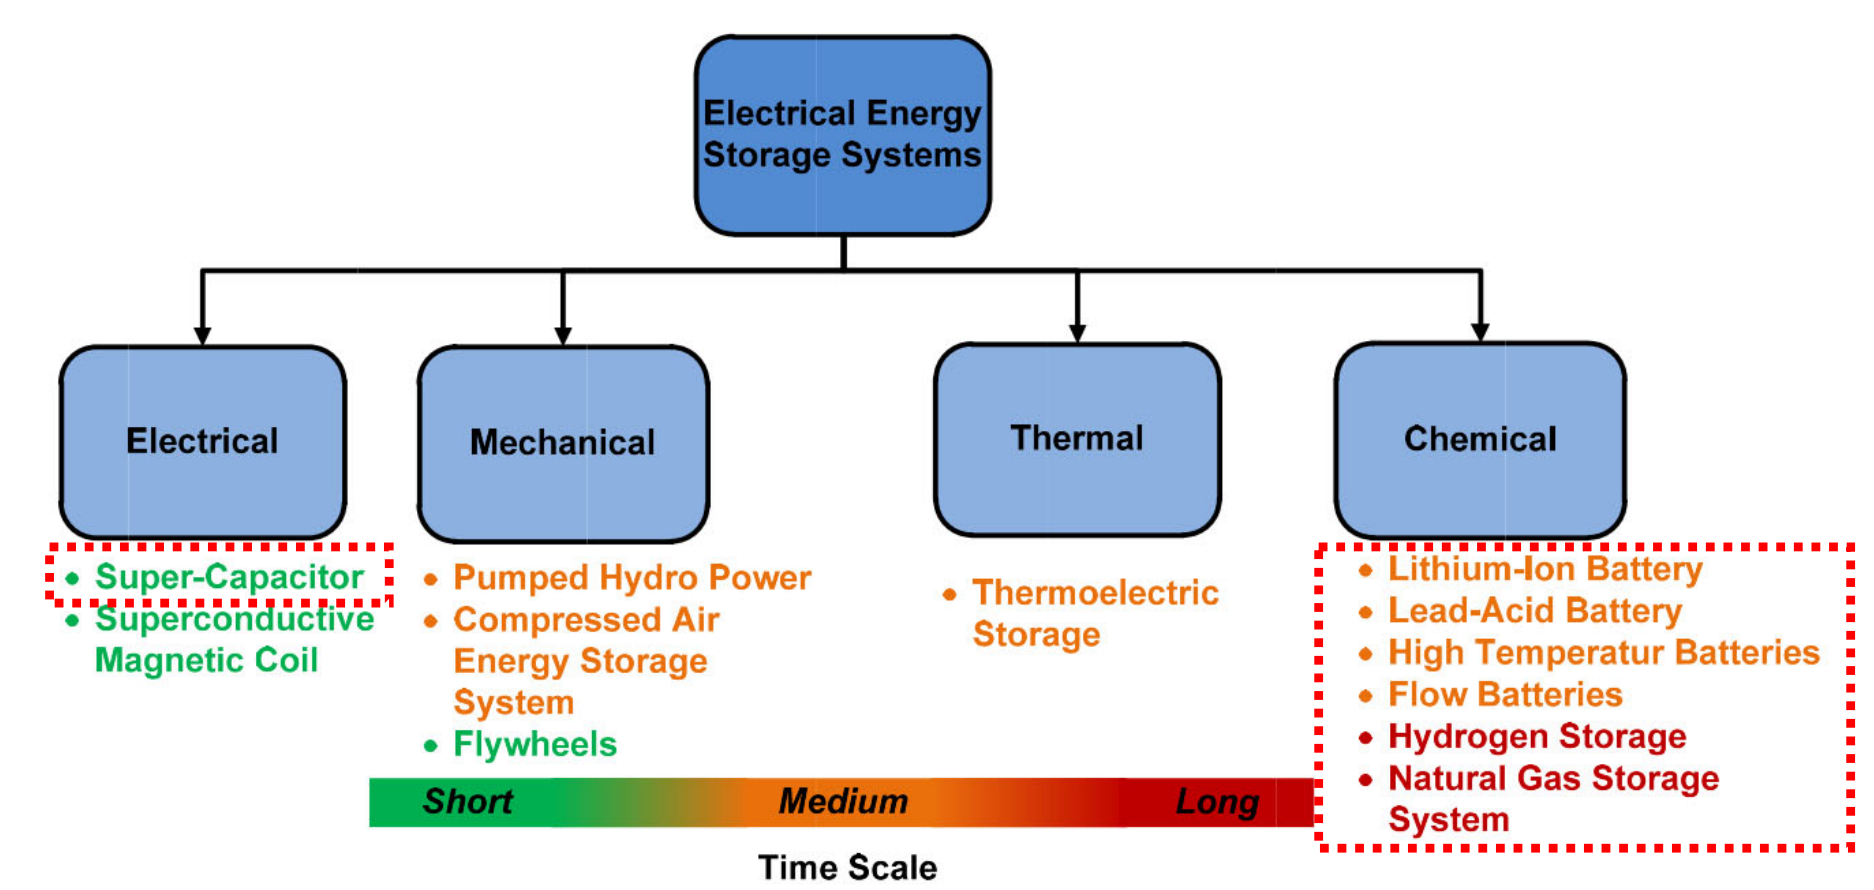
\includegraphics[width=\linewidth]{src/overview.png}
    \label{fig:enter-label}
\end{figure}
\vspace{-1cm}
primary energy consumption 2021: 595 EJ/a = 165 PWh/a = 19 TW
30\% of elec. production from renewables. pimary energy vs. final energy CH: 280 / 221 TWh.
\subsection{Technologies overview}
\begin{figure}[H]
    \centering
    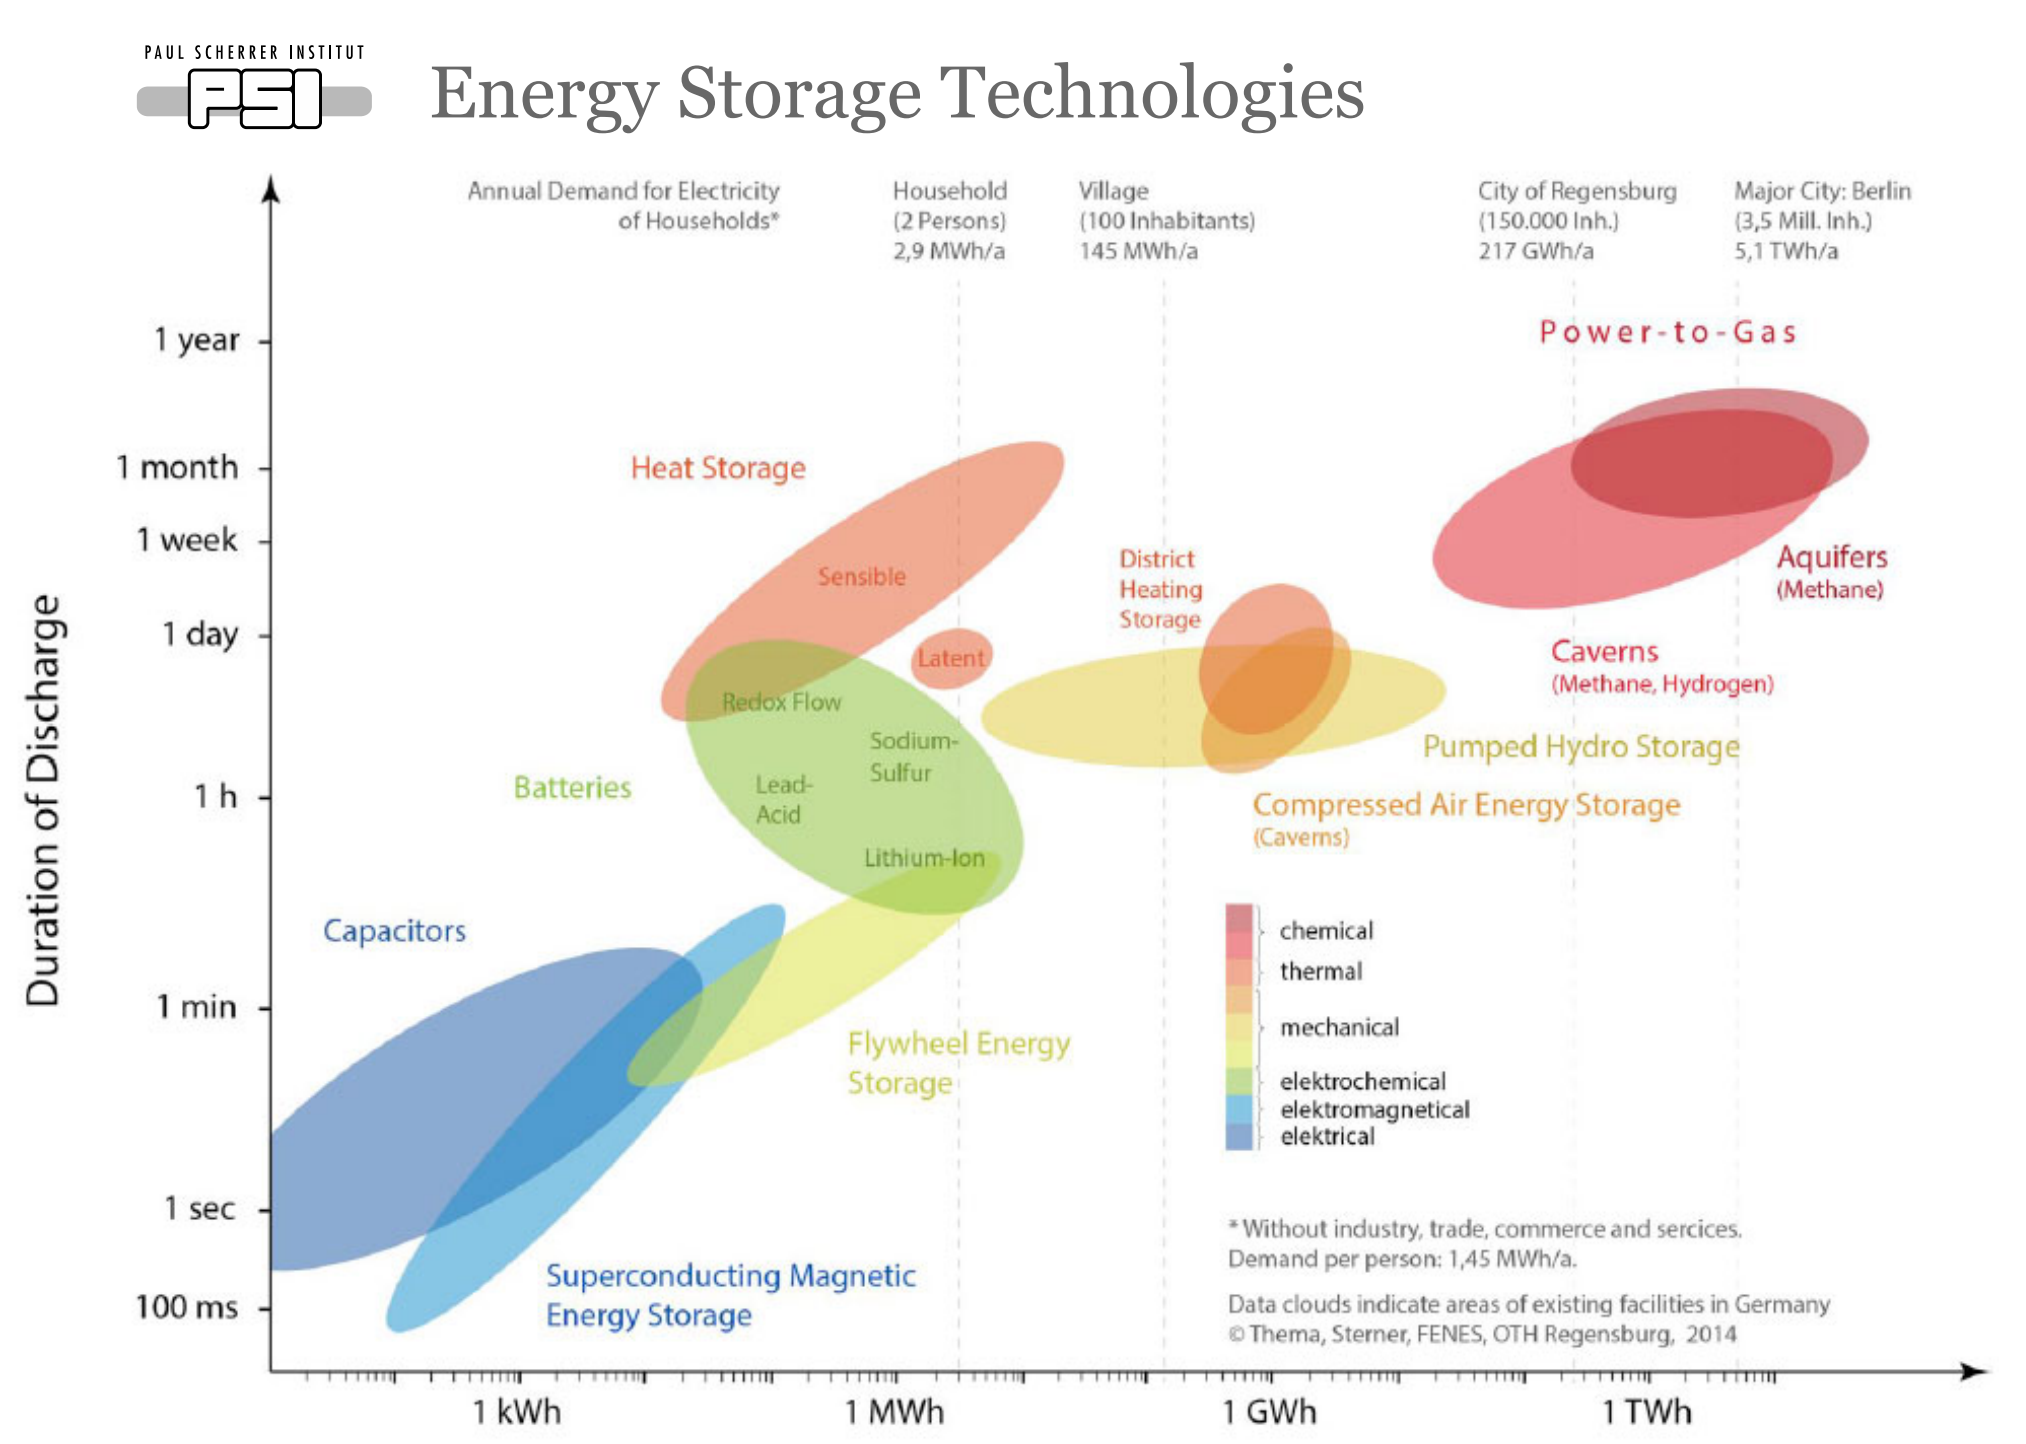
\includegraphics[width=.8\linewidth]{src/tech_ow.png}
    \label{fig:tech_ow}
\end{figure}
\subsection{LCOE}
$$
\begin{aligned}
\mathbf{L C O E} & =\frac{\text { total cost over lifetime }}{\text { total electricity generated }} \\ 
& =\frac{\sum_{t=1}^n\left(I_t+M_t+F_t+R_t\right) \cdot(1+r)^{-t}}{\sum_{t=1}^n E_t \cdot(1+r)^{-t}} \\
& =\frac{\sum_{t=1}^n\left(\frac{I_t+M_t+F_t+R_t}{\mathrm{MW}}\right) \cdot(1+r)^{-t}}{\sum_{t=1}^n t\cdot \mathrm{\frac{hours}{t}}\cdot \frac{\%}{100}_\mathrm{cap} \cdot(1+r)^{-t}} \quad \mathrm{\left[\frac{EUR}{MWh}\right]}
\end{aligned}
$$
with $F_t, R_t$ fuel/recycling cost in year $t$ (in EUR), $E_t$: $\mathrm{MWh}$ energy gen. in year $t$, $\frac{\%}{100}_\mathrm{cap}$ the capacity factor. \\
LCOE for renewbales have been falling dramtically compared to fossil fuels in recent years.

\section{Electrochemistry}
chemical reactions + transfer of electric charges\\
i.e., interaction electrical energy $\Leftrightarrow$ chemical change. \\
reactions are redox reactions, i.e. the oxidation \# changes
\subsection{quantities}
\textit{Energy E} is the capacity of a physical system to perform work\\
\textit{Heat Q}: most dispersed form of energy \\
\textit{Work W}: useful energy \\
\textit{Power P}: energy converted / heat released /  work performed per unit time. $E=\int Pdt$
\subsection{thermodynamic state functions}
thermodynamic state functions and ideal cell voltage
(= thermodynamic potentials*, subscript ‘r’ = ‘reaction’):
\vspace{-.5cm}
\begin{figure}[H]
    \centering
    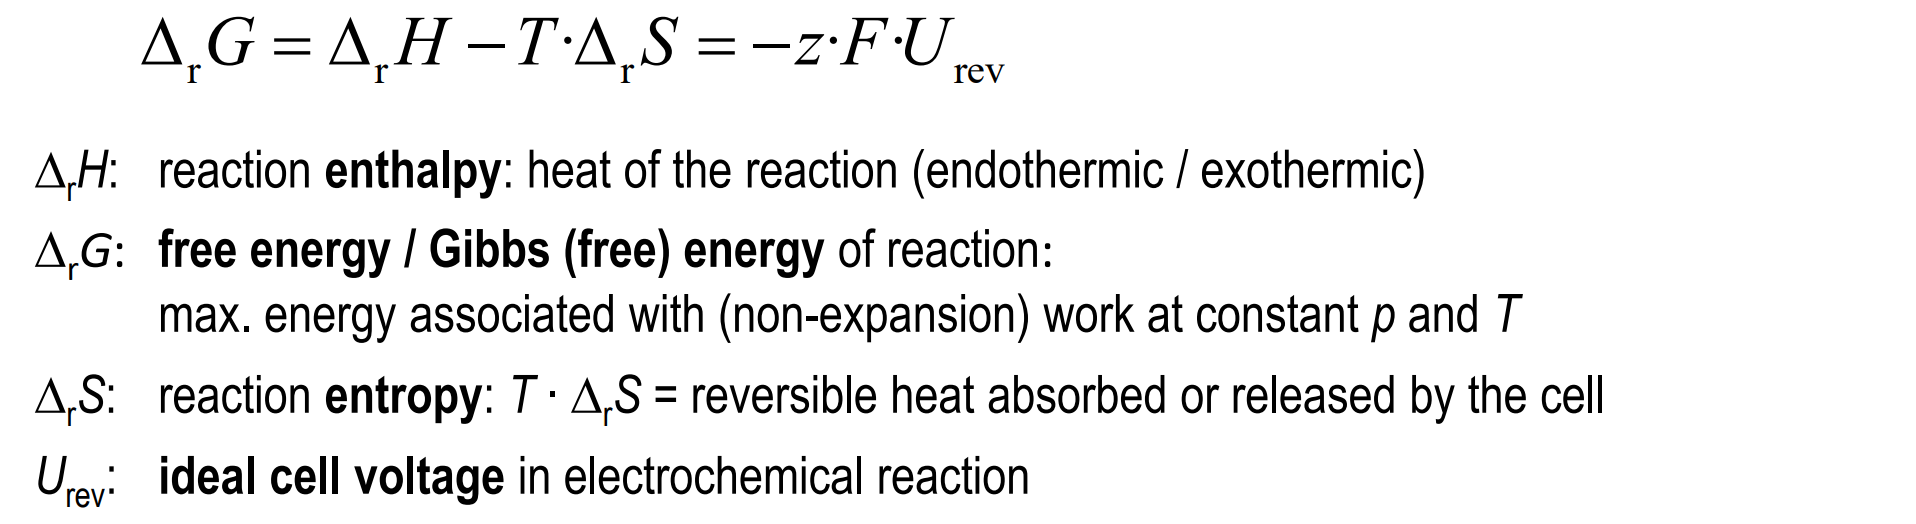
\includegraphics[width=1\linewidth]{src/gibbs_1.png}
    \label{fig:gibbs_1}
\end{figure}
\vspace{-1cm}
solving this:
\begin{enumerate}
    \item calculate reaction enthalpy: $\Delta_{\mathrm{r}} H^{\circ}=\sum v_{\mathrm{i}} \cdot \Delta_{\mathrm{f}} H_{\mathrm{i}}^{\circ}$
    \item calc. reaction entropy: $\Delta_{\mathrm{r}} S^{\circ}=\sum v_{\mathrm{i}} \cdot S_{\mathrm{i}}^{\circ}$
    \item assemble free energy of rxn: $\Delta_{\mathrm{r}} G^{\circ} = \Delta_{\mathrm{r}} H^{\circ}- T\Delta_{\mathrm{r}} S^{\circ}$
\end{enumerate}
note:
\begin{itemize}
\item $\Delta_{\mathrm{r}} G^{\circ}> 0$: non-spontaneous (electrolytic cell)
\item $\Delta_{\mathrm{r}} G^{\circ}<0$: spontaneous (galvanic cell)
\end{itemize}
% table for example
\begin{tabular}{|c|c|c|c|c|}
\hline
\textbf{Quantity} & \textbf{Units} & \textbf{H\textsubscript{2}} & \textbf{O\textsubscript{2}} & \textbf{H\textsubscript{2}O(l)} \\ \hline
$\Delta_fH^\circ$ & kJ/mol        & 0    & 0    & -285.8  \\ \hline
$S^\circ$        & J/(mol·K)      & 130.7 & 205.1 & 69.9    \\ \hline
$\Delta_fG^\circ$ & kJ/mol        & 0    & 0    & -237.1  \\ \hline
\end{tabular}
\section{E-Chem cell}
\begin{figure}[H]
    \centering
    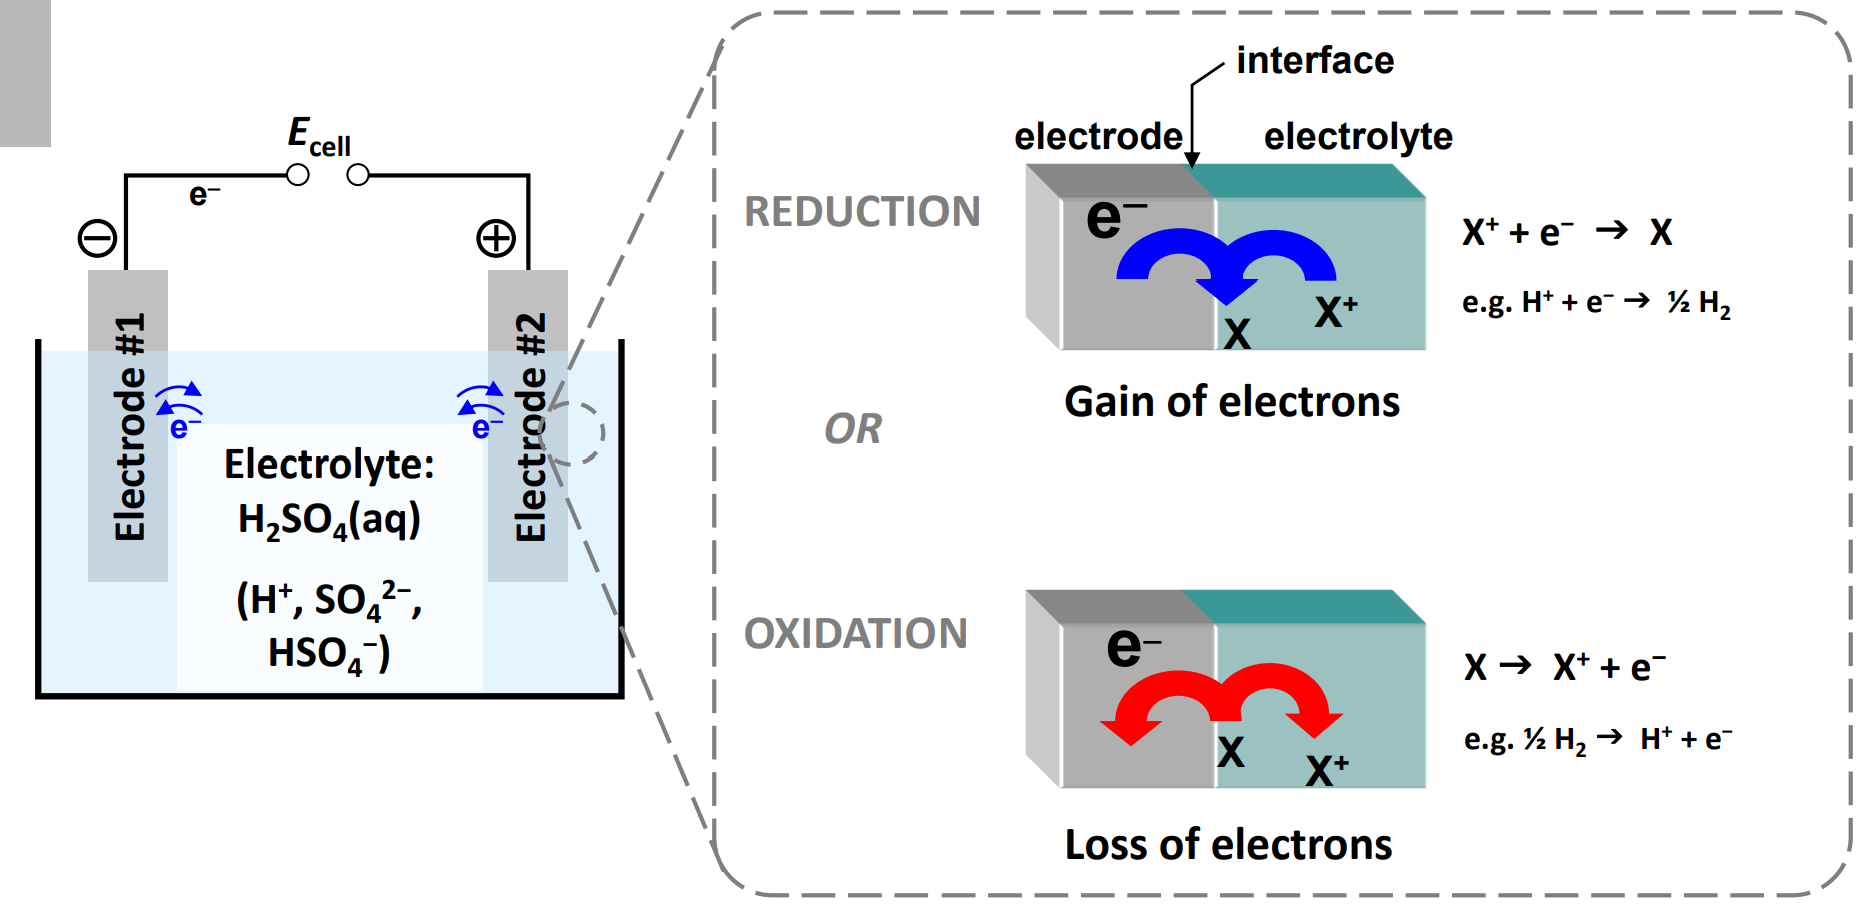
\includegraphics[width=1\linewidth]{src/e_cell_redox.png}
    \label{fig:e_cell_redox}
\end{figure}
\vspace{-1cm}
\begin{itemize}
    \item redox reaction on each electrode
    \item each electride has given potential $E$
    \item $e^-$ transferred via conductor and electrode-electrolyte interface
    \item ions transferred through electrolyte
\end{itemize}
\subsection{equilibrium}
open circuit, i.e. electrodes not connected. rate of reduction vs. oxidation is equal. no net current flow. problem: we cannot easily measure potential. thus we define: \\
$$ E^0=-\frac{\Delta G^0}{z \cdot F}=-\frac{\Delta H^0-T \cdot \Delta S^0}{z \cdot F}$$
$x^0$ indicates standard conditions ($T=25^\circ$C,$p=1$ atm). $z :=$ \#electrons, $F:=$ Faraday const., $\Delta G^0$ useful energy. \\
$E^0(2H^+ +2e^-\Rightarrow H_2)=V_{H_2}-SHE=0$ by def. \\
What does $E^0$ mean? \\
\vspace{-.5cm}
\begin{itemize}
    \item high $\Rightarrow$ tendency to get reduced ("oxidizing agent")
    \item low $\Rightarrow$ tendency to get oxidised ("reducing agent")
\end{itemize}
\vspace{.2cm}
$$E_{cell}=E_{pos}-E_{neg}$$
\begin{itemize}
    \item if $E_{cell}>0$, reaction spontaneous and vice versa
\end{itemize}

\subsubsection{cell notation}
$|=$ phase boundary, 
$||$ = salt bridge \\
$\vdots =$ liquid junction (separator) $\vdots\vdots =$ semipermeable membrane \\
example "Daniell cell": 
$$\mathrm{Zn|Zn_{2+},SO_4
^{2-}(aq)||Cu^{2+},SO_4
^{2-}(aq)|Cu}$$

\subsection{standard $\mathrm{H_2}$ electrode}
piece of Pt comes in contact with a solution containing $\mathrm{H^+}$ under thermodynamically reversible conditions at unit activity

\subsection{The Nernst equation}
\begin{tabular}{|p{.6cm}|p{2cm}|p{2cm}|p{3cm}|}
\hline
        & gases & ionic species & solids or w.i.e. \\

$a_i=$   & $p_i\mathrm{[atm]}$ & $C_i \mathrm{\left[\frac{mol}{L}\right]}$ & 1 \\

e.g. & $\mathrm{H_2,O_2}$ & $\mathrm{Cu^{2+},x^{-}}$ & $\mathrm{H_2O}$ \\
\end{tabular}
w.i.e. = water in electrolytes
\subsubsection{half reaction}
let $a\cdot A+z\cdot e^-\leftrightarrow c\cdot C$:
$$E_{rev}=E^0+\frac{R \cdot T}{z \cdot F}\ln \left(\frac{a_A^a}{a_C^c}\right)$$

\subsubsection{full reaction}
for non-standard conditions, let $aA+bB\leftrightarrow cC+dD$:
$$
E_{r e v}=E^0+\frac{R \cdot T}{z \cdot F} \ln \left(\frac{a_A^a \cdot a_B^b}{a_C^c \cdot a_D^d}\right)
$$
\vspace{-.3cm}
% \begin{itemize}
%     \item for gases, $a_i = p_i$ [atm]
%     \item for ionic species, $a_i = C_i$ [mol/L] \\
%     \item for solids or water in aqueous electrolytes, $a_i=1$
% \end{itemize}
\subsubsection{example: Danniell cell}
at $T = 298 K,
C(Zn^{2+}) = 10^{-3} \mathrm{M}$ and $ C(Cu^{2+}) = 10^{-6} \mathrm{M}$:
\vspace{-.3cm}
\begin{align*}
    E_{\text {rev }} & =E^0+\frac{R \cdot T}{z \cdot F} \ln \left(\frac{a_A^a \cdot a_B^b}{a_C^c \cdot a_D^d}\right)=1.10+\frac{8.314 \cdot 298}{2 \cdot 96485} \\
    & \cdot\ln \left(\frac{10^{-6}}{10^{-3}}\right) = 1.01 \mathrm{V}
\end{align*}
\vspace{-.5cm}

\subsubsection{example: oxygen reduction reaction (ORR)}
at pH 1, $T = 298 K, p(\mathrm{O_2})=1$ atm: \\
$\mathrm{O_2+4H^+ + 4e^- \rightarrow 2H_2O} \quad E^0=1.23 \mathrm{V}$ \\
$a_{\mathrm{H^+}}\approx.1\Rightarrow\mathrm{ph}=-\log_{10}{a_{\mathrm{H^+}}}$: $E=1.23\mathrm{V} - 0.059=1.171 \mathrm{V}$

\subsection{Potential vs. pH relations: the Pourbaix diagram}
basically a plotting method of the Nernst equation. we derive $\mathrm{pH}=\log_{10}\left(\frac{1}{a_{H^+}}\right)$ \\
we can use it to "predict" a material’s
behaviour in aqueous electrolytes
as a function of E and pH.
\vspace{-.5cm}
% \begin{figure}[H]
%     \centering
%     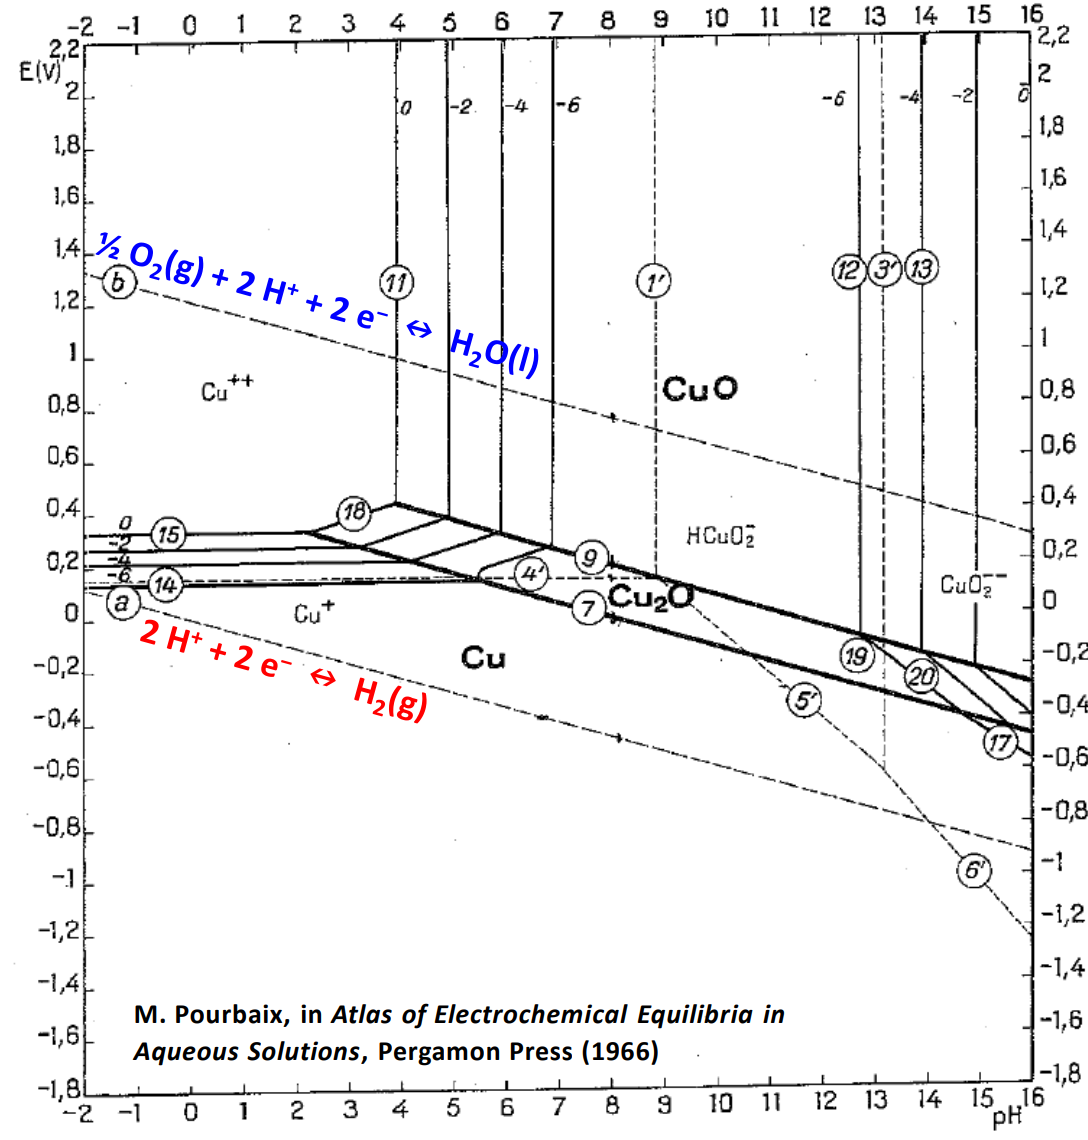
\includegraphics[width=0.5\linewidth]{src/pourbaix.png}
% \end{figure}
% \begin{figure}[H]
%     \centering
%     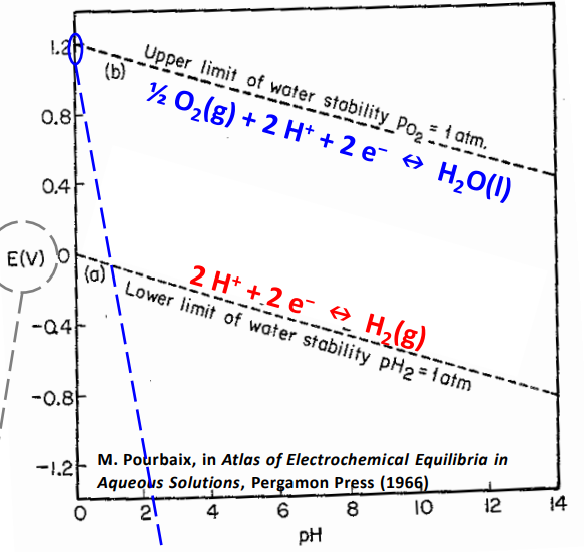
\includegraphics[width=1\linewidth]{src/pourbaix2.png}
% \end{figure}
\begin{figure}[H]
    \centering
    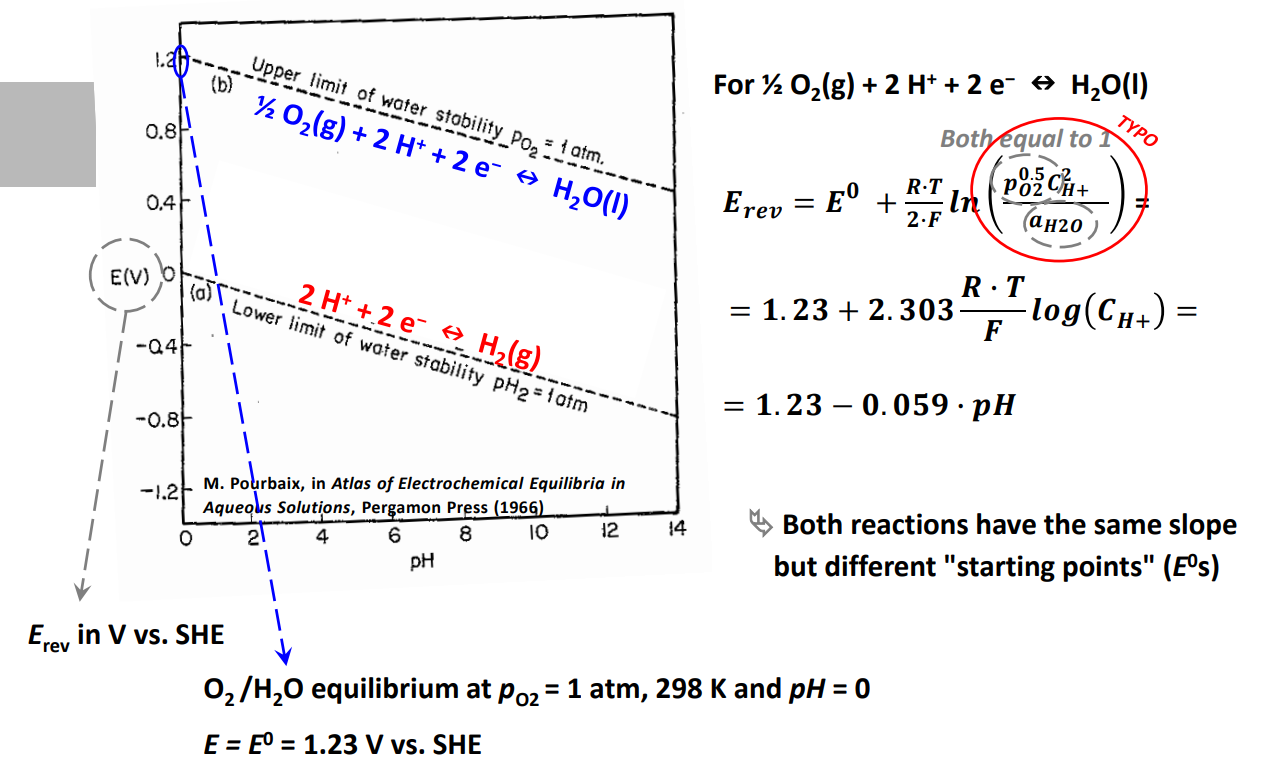
\includegraphics[width=1\linewidth]{src/purbaix_full.png}
\end{figure}
\vspace{-1cm}

\subsection{E-Chem. cell overview}
\begin{figure}[H]
    \centering
    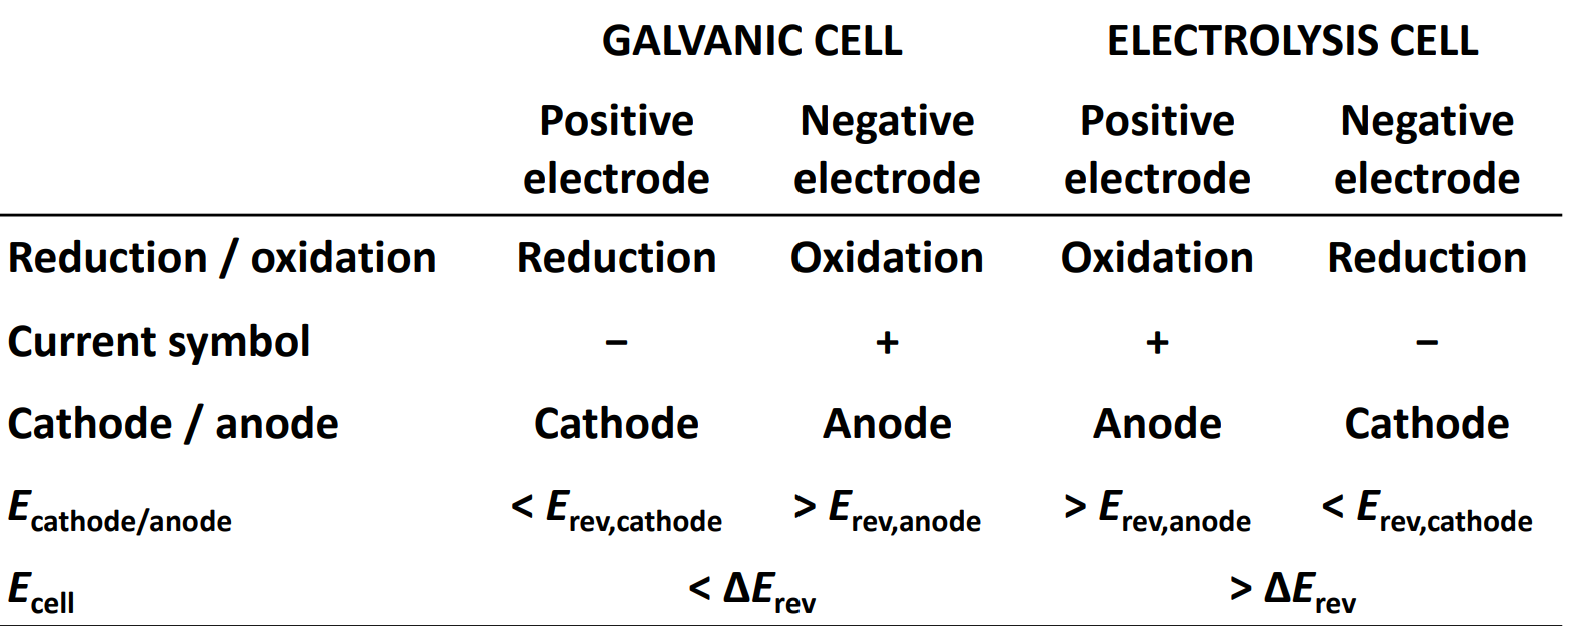
\includegraphics[width=1\linewidth]{src/cells_comp.png}
\end{figure}
\vspace{-.3cm}

\subsection{Galvanic cell}
% \begin{figure}[H]
%     \centering
%     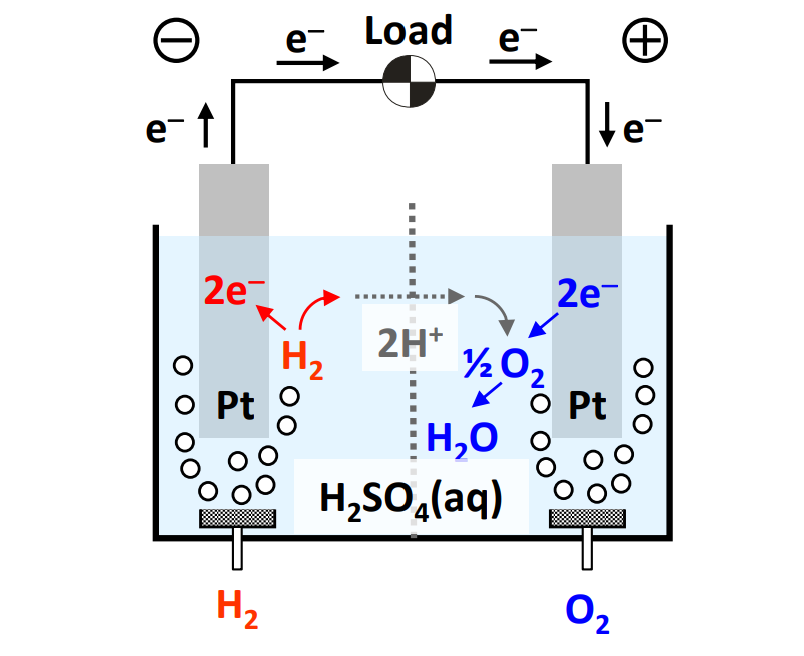
\includegraphics[width=0.5\linewidth]{load_cell.png}
% \end{figure}
lets assume we connect a load between the conductors $\Rightarrow$ spontaneous reactions take place.
\begin{figure}[H]
    \centering
    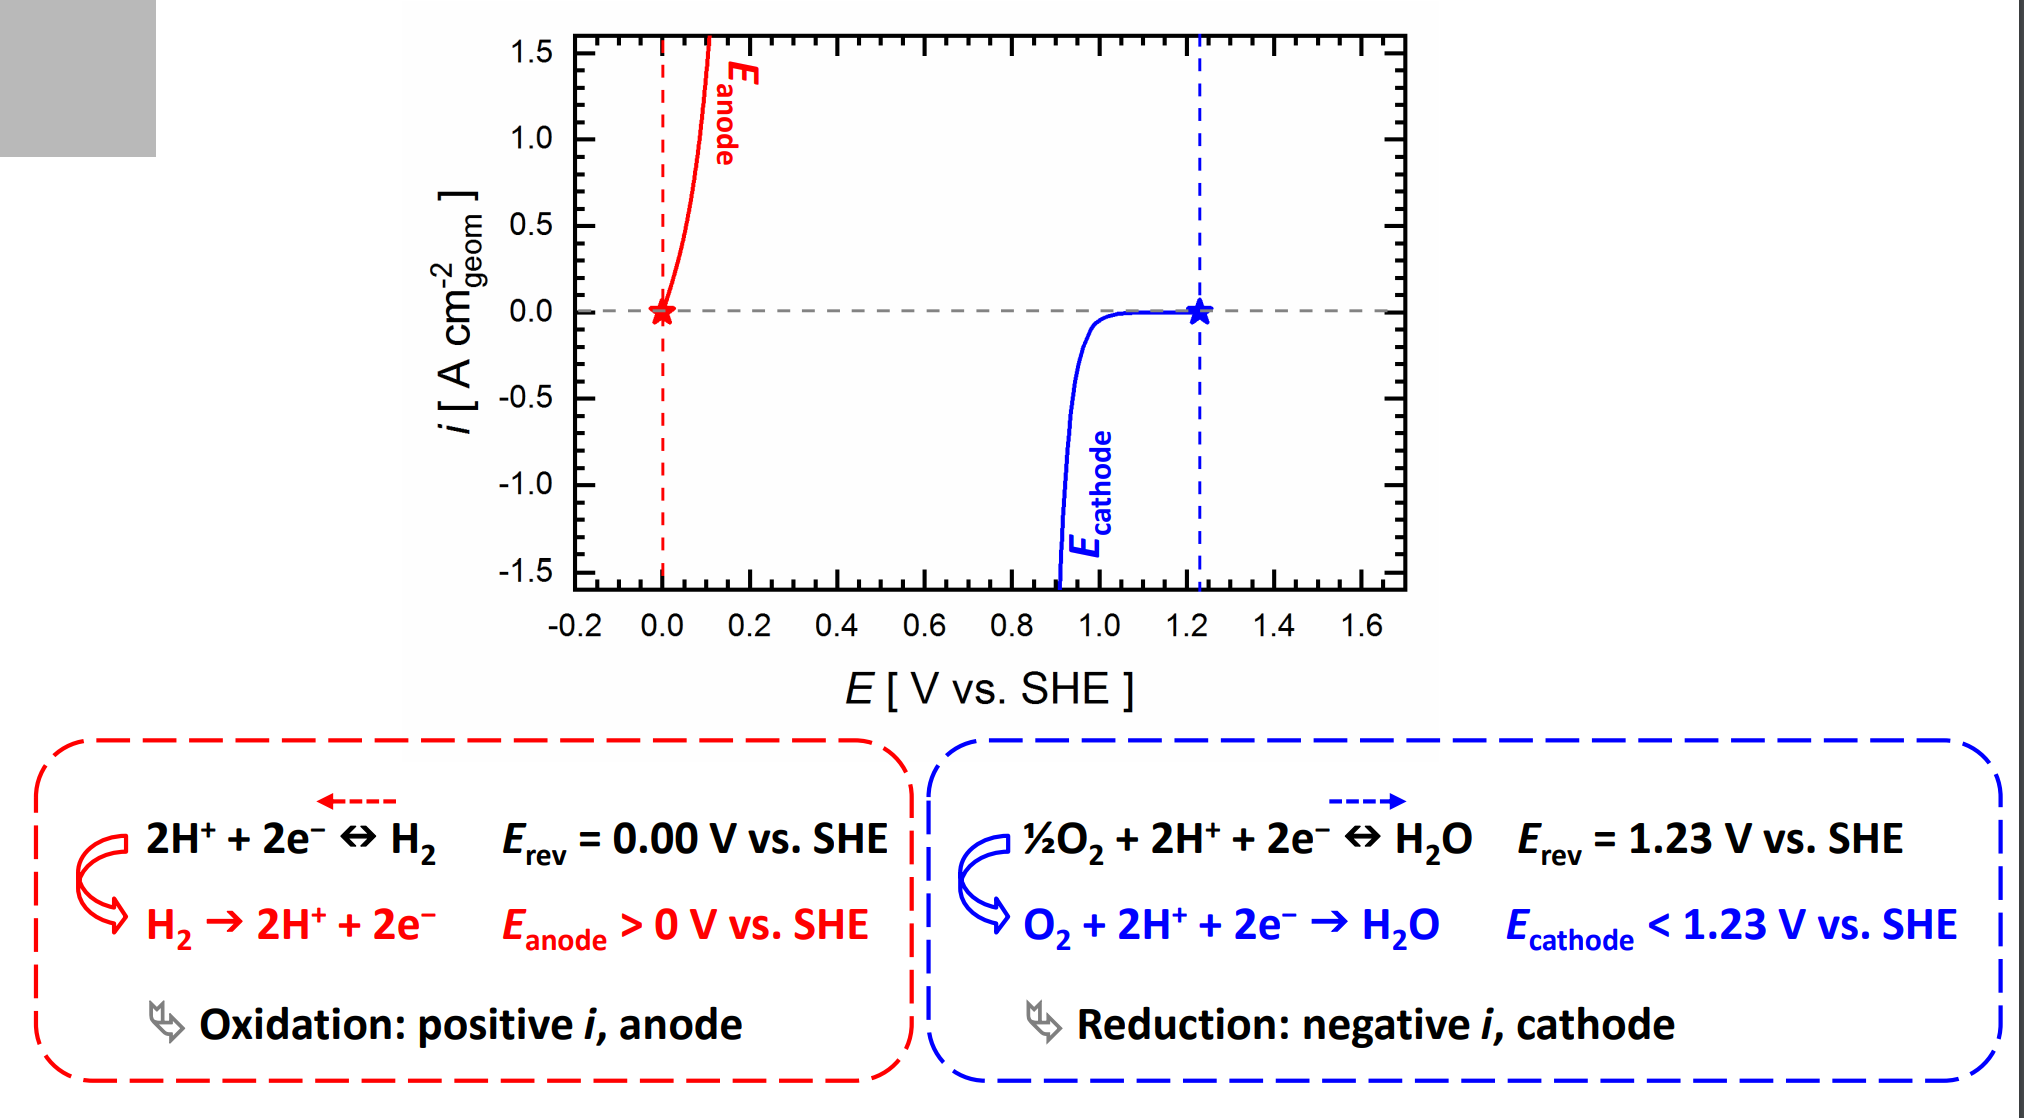
\includegraphics[width=1\linewidth]{src/galvanic.png}
\end{figure}
\vspace{-.6cm}
in a galvanic cell $E_{cell}<\Delta E_{rev}$.\\
$E_{cell}=E_{pos}-E_{neg}=E_{cath}-E_{anode}$\\
$\approx .8V$ for this example

\subsection{The Electrolysis cell}
connecting a voltage source of $E>\Delta E_{rev}$ drives the non-spontaneous reactions:
\begin{figure}[H]
    \centering
    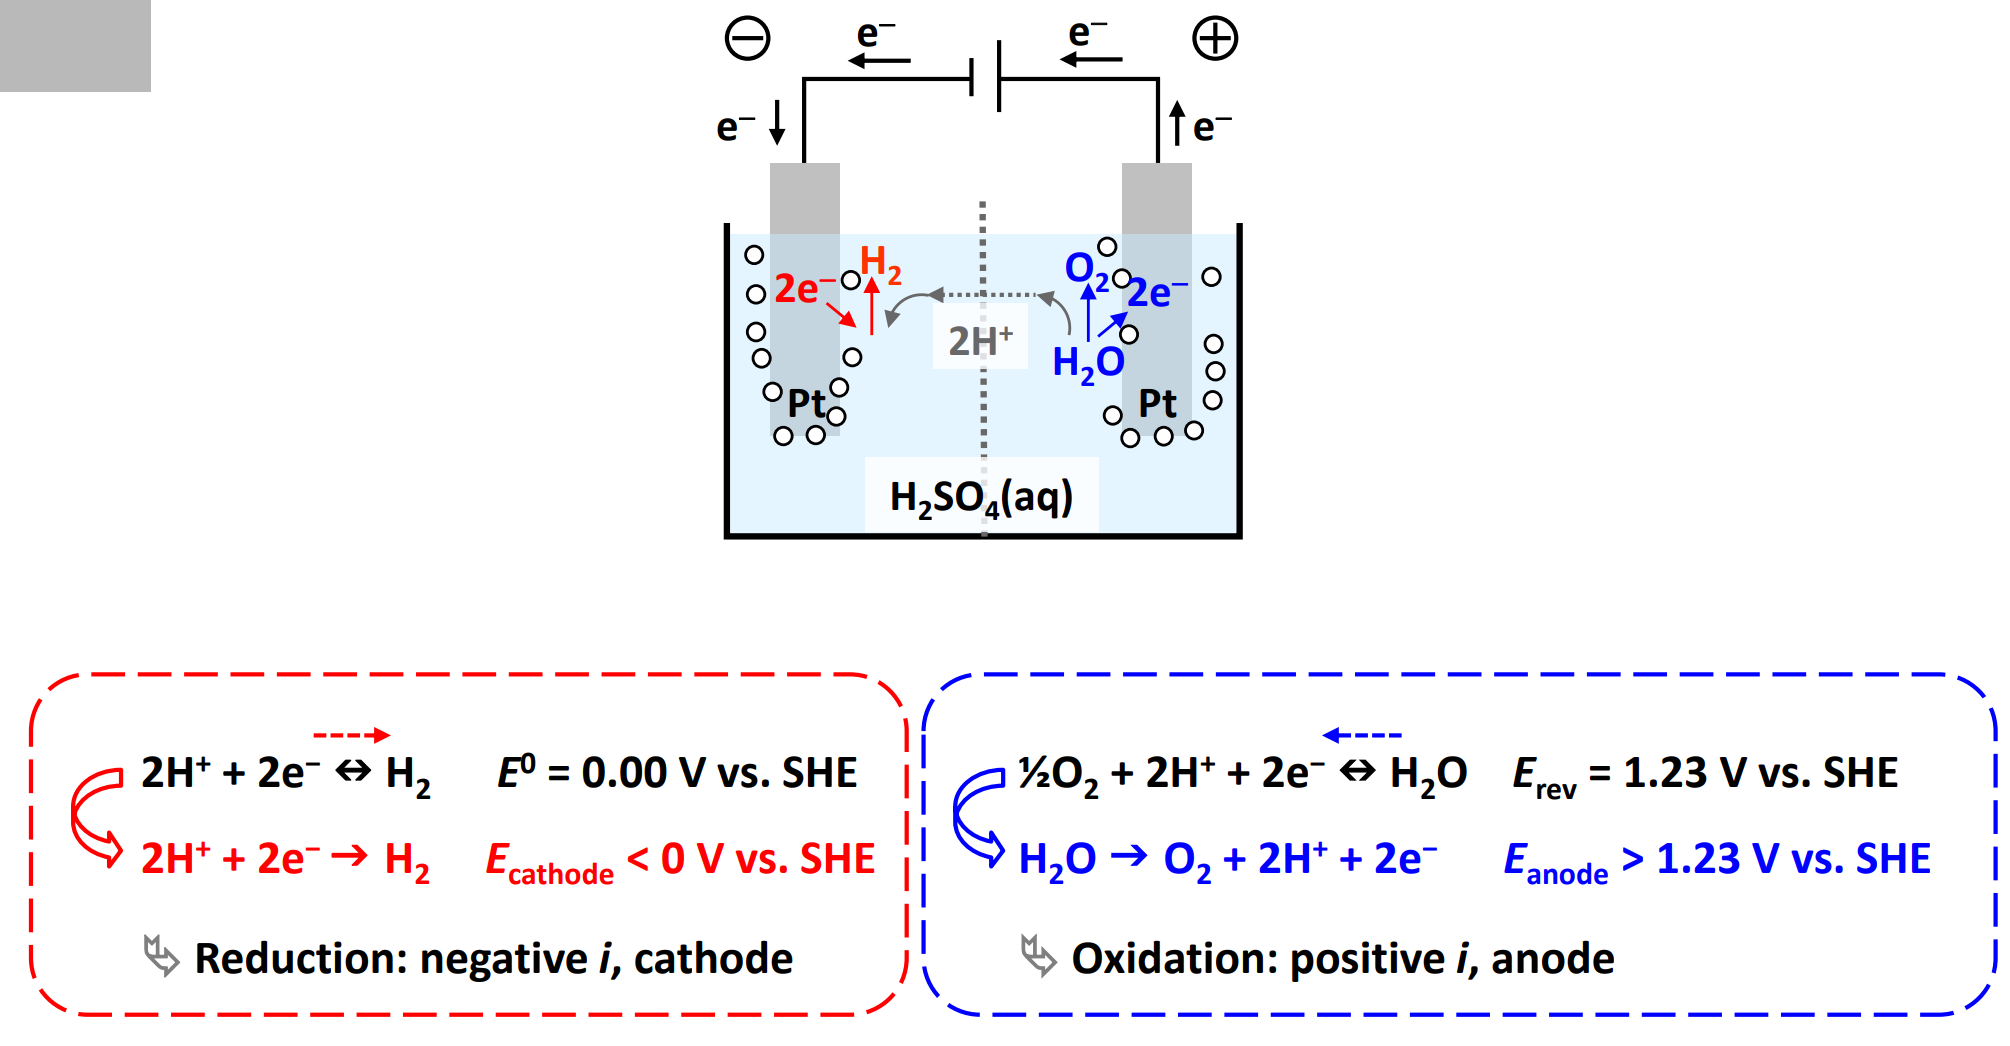
\includegraphics[width=\linewidth]{src/electrolysis_cell.png}
\end{figure}
\vspace{-.5cm}
\begin{figure}[H]
    \centering
    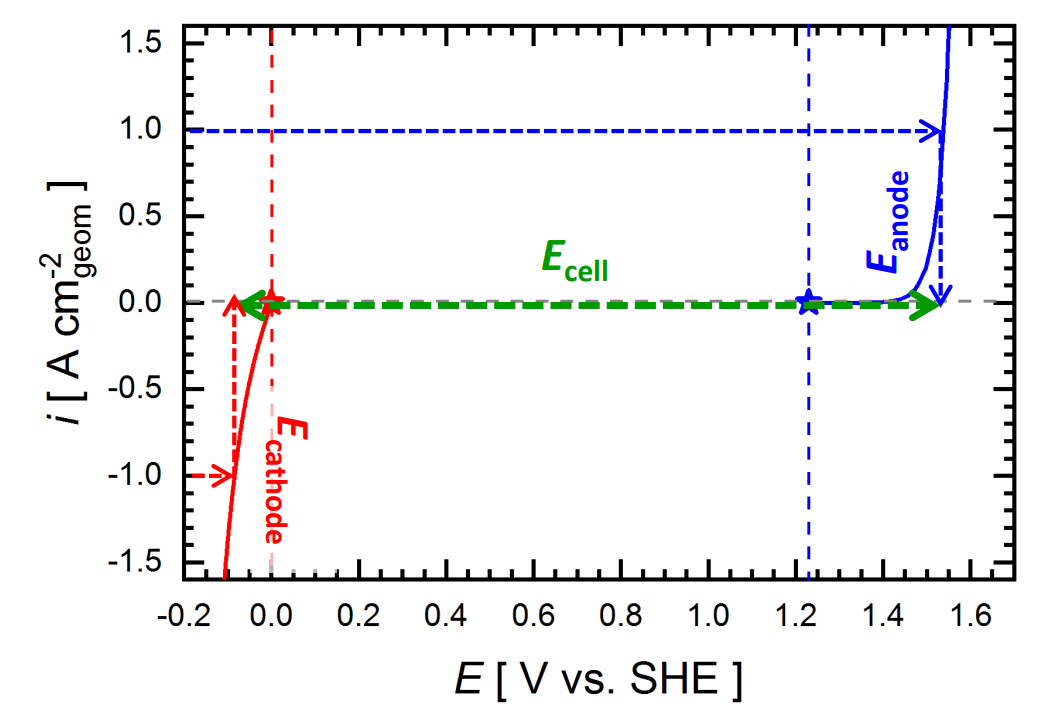
\includegraphics[width=.7\linewidth]{src/electrolysis_cell_pot.png}
\end{figure}
\vspace{-.5cm}
thus in electrolysis cell we have
$$E_{cell}>\Delta E_{rev}$$
and for this example $E_{cell}=E_{anode}-E_{cathode}\approx 1.6V$

\subsection{Faraday's Law}
using $Q=z\cdot F\cdot n$ 
$$I(t)=\frac{\delta Q}{\delta t}=z\cdot F\cdot \frac{\delta n}{\delta t}= z\cdot F\cdot r$$
with $n$ \# $[\mathrm{mol}]$, $r$ the reaction rate in $\left[\mathrm{\frac{mol}{s}}\right]$, $F=96 485 \left[\mathrm{\frac{A\cdot s}{mol}}\right]$ 
\subsection{over-potential}
$$\eta =E-E_{rev}$$
is the \textbf{over-potential} quantifying the deviation thermodynamic potential and half reactions potential.\\
positive for oxidation, negative for reduction. \\
$$\eta_{tot}=\eta_{mtx}+\eta_R+\eta_{kin}$$
where 
\begin{itemize}
    \item Mass transport (mtx): $O_2$ and $H_2O$ need to be transported to and away from the electrode
    \item  Ohmic (R): transport of $H^+$s and $e^-$s with an associated resistive loss
    \item Kinetics (kin): catalytically demanding reaction
\end{itemize}

\subsection{Butler-Volmer Equation}
$$
i_{\text {kin }}=i_0 \cdot R F \cdot\left[\underbrace{\exp \left(\frac{\alpha_a \cdot F}{R \cdot T} \cdot \eta_{k i n}\right)}_{anodic}+\underbrace{-\exp \left(-\frac{\alpha_c \cdot F}{R \cdot T} \cdot \eta_{k i n}\right)}_{cathodic}\right]
$$
depending on $\left(T, C_i\right)$, where
\begin{itemize}
    \item $i_{kin}$ is the current under purely kinetic control
    \item $i_0$ is the (exchange) current at zero over-potential
    \item $RF=\frac{A_{\text{catalyst}}}{A_{\text{geometry}
    }}$ is the roughness factor
    \item $\alpha_{a,c}$ are the anodic and cathodic transfer coeff.
    \item $F,R,T$ faradays const, gas const., temp.
\end{itemize}

\begin{figure}[H]
    \centering
    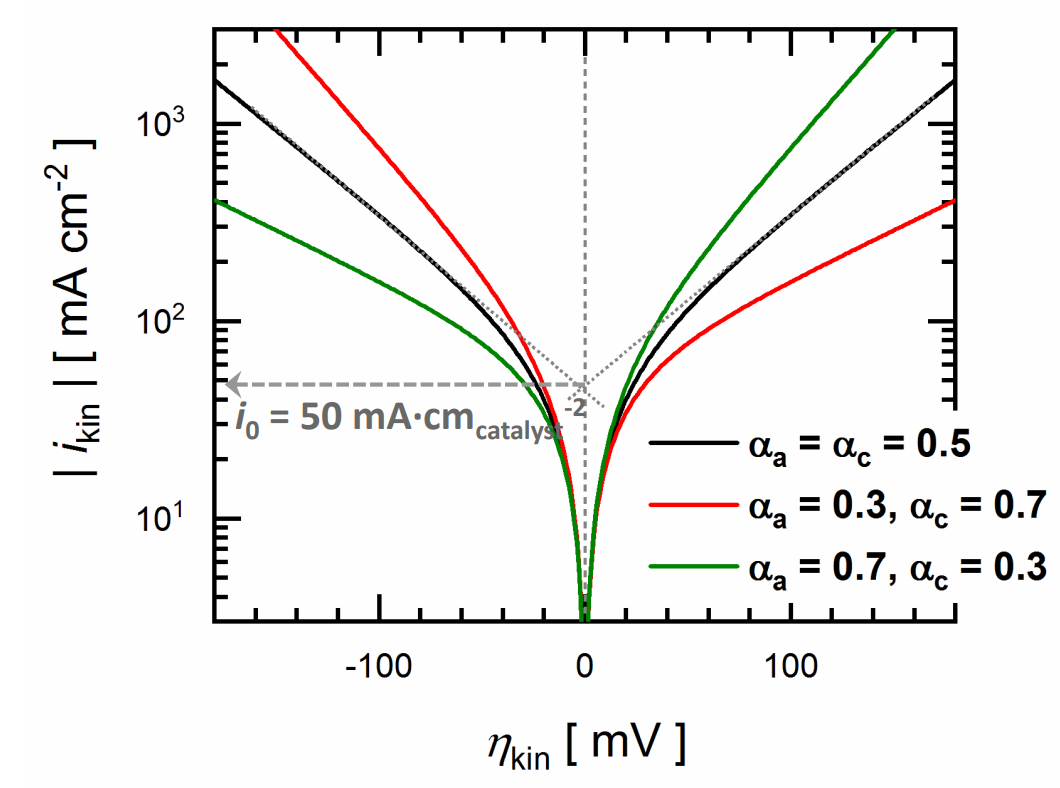
\includegraphics[width=.7\linewidth]{src/butler1.png}
\end{figure}
larger $\alpha$'s lead to greater slopes $\Rightarrow$ smaller $\eta$ increases leads to larger $i_{kin}$ \\
If one of terms neglected:
$$\eta=\ln\left(\frac{i_{kin}}{i_0\cdot RF}\right)\cdot\frac{R\cdot T}{\alpha_{a/c} F}$$

\subsection{Tafel Equation}
At high overpotentials, the contribution of the reverse reaction to the total current becomes negligible. Thus we can approximate:
$$
i_{\text {kin }}\left(T, C_i\right)=i_0\left(T, C_i\right) \cdot R F \cdot\left[\underbrace{10^{\eta / b_a}}_{i_{anodic}}+\underbrace{-10^{-\eta / b_c}}_{i_{cathodic}}\right]
$$
with $b_{a/c}=\frac{2.3\cdot RT}{\alpha_{a/c}F}$ \\
can neglect $i_{a}$ or $i_{c}$ depending on $\pm\eta>\frac{b_{a/c}}{2}$ : \\
$\log_{10}{\frac{i_{kin}}{i_0\cdot RF}}=\eta/b_{a/c}$, thus
$$\eta\propto b_{a/c}\cdot \log_{10}(i_{kin})$$
where $b_{a/c}=\ln(10)\cdot\frac{R\cdot T}{F\cdot \alpha_{a/c}}$ is the Tafel slope.
\subsubsection{example: Pt-based electrode}
$\mathrm{RF}=200\mathrm{\frac{cm_{Pt}^2}{cm^2_{geom}}}$, operating $\mathrm{O}_2$ reduction at 0.9V vs SHE. Assuming standard conditions, exchange current density of $i_0=5\cdot 10^{-10}\mathrm{\frac{A}{cm_{Pt}^2}}$ and $\alpha_a,\alpha_c=1$, calculate $i_{kin}$: \\
$\eta=E-E_{rev}=0.9-1.23=-0.33$ V\\
tafel slope: $b_c=\frac{2.3\cdot R\cdot T}{\alpha_c F}=0.059$ V \\
since $\eta>b_c/2$, we can estimate: \\
$i_{kin}=i_0\cdot RF\cdot [-10^{-\eta/b_c}]=-0.039  \mathrm{\frac{A}{cm_{geom}^2}}$

\subsection{Mass transport}
limitations are:
\begin{itemize}
    \item Migration: charged body moving due to an electric field
    \item Diffusion: species moving due to a concentration gradient
    \item Convection: stirring or hydrodynamic transport
\end{itemize}
\textbf{But} In most practical cases, electrolyte solutions are concentrated enough for migration to become negligible. \\
However, a concentration gradient between surface and bulk can lead to a build up diffusion of thickness $\delta_{DL}$. at high over-potentials $c_{surface}=0$ and $i=i_{lim}$, thus
$$\frac{i_{lim}}{z\cdot F}=\frac{D}{\delta_{DL}}c_{bulk}$$
the issue is $\delta_{DL}$ is ill defined therefore rotating disk electrodes are used to find analytical solutions to $\delta_{DL}=f(D,\text{viscosity, electrode rotation})$\\
as a first approximation we can thus yield
$$\frac{1}{i}=\frac{1}{i_{kin}}+\frac{1}{i_{lim}}$$
\subsection{Electrolyte}
\textit{Ohmic losses mostly arise from the electrolyte’s conductivity} \\
in the electrolyte we must have $i_{elec}=i_{ion}$. the ion condution is set by:
\begin{itemize}
    \item Charge and radius of the (solvated) ions
    \item ionic concentration
    \item electrolytes viscosity 
    \item cell's dimension (areas, inter-electrode distance)
\end{itemize}
conductivity $\sigma=\frac{1}{\rho}=\frac{L}{A\cdot R}$ \\
thus $R_a=R\cdot A= \frac{L}{\sigma}$ the areal resistance, the ohmic over-potential is:
$$\eta_R=i\cdot R_a$$
using an approximation for dilute solutions: $\sigma=\Lambda_m\cdot c$
Kolhrausch's law is derived: $\Lambda_m=\Lambda_m^0 - A\sqrt{c}$
with $\Lambda_m$ decreasing due to overlap of hydration spheres. \\
$\Lambda_m^0=n\lambda_+ + m\lambda_-$ where $\lambda_{+/-}$ are the molar conductivity of single ions [$\frac{S\cdot cm^2}{mol}$]

\subsection{total $i$ vs. $E$ curve}
\begin{figure}[H]
    \centering
    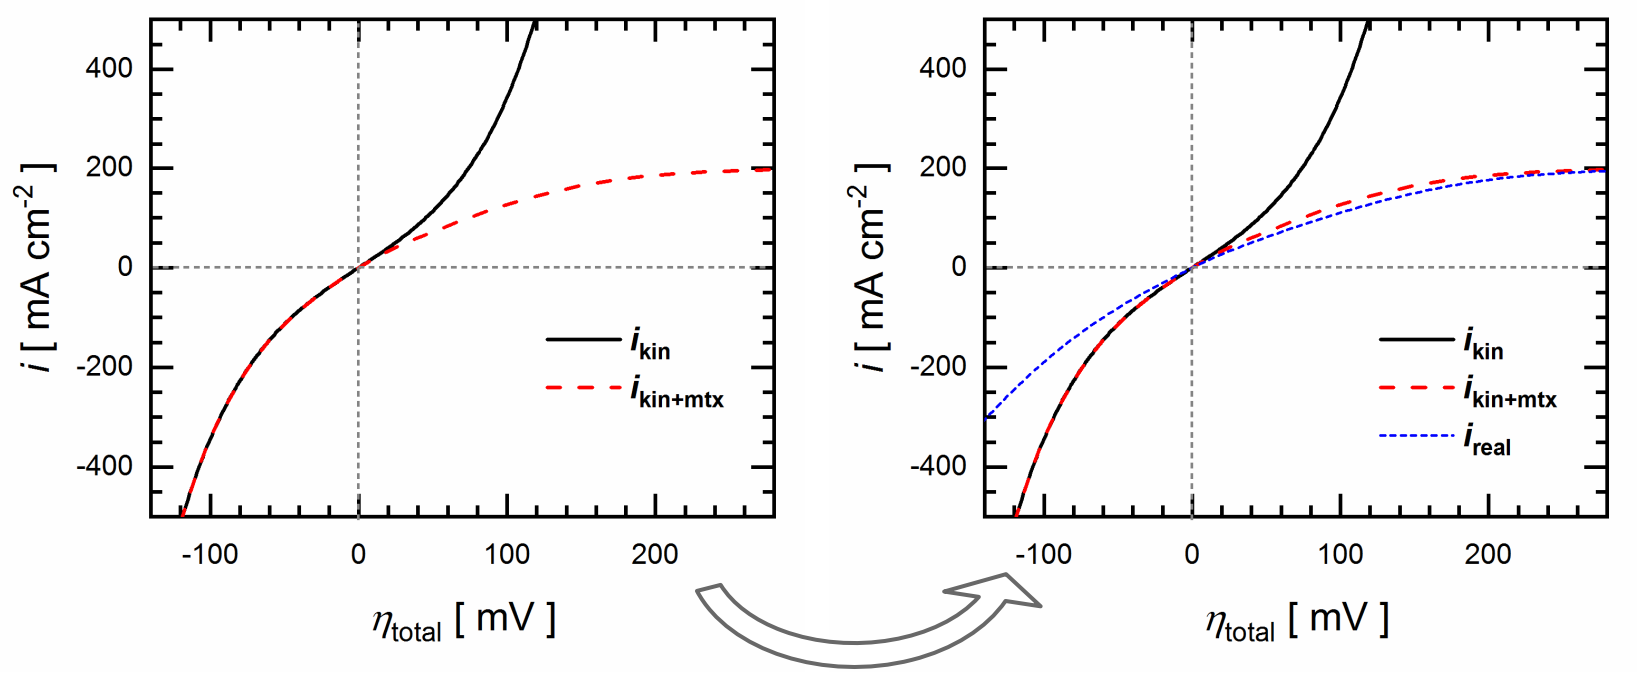
\includegraphics[width=1\linewidth]{src/iE_full.png}
\end{figure}

\section{Hydrogen}
motivation: \textit{could} be 1) produced from RE, 2) used as energy carrier, 3) be carbon free and 4) cover wide range of applications
\begin{figure}[H]
    \centering
    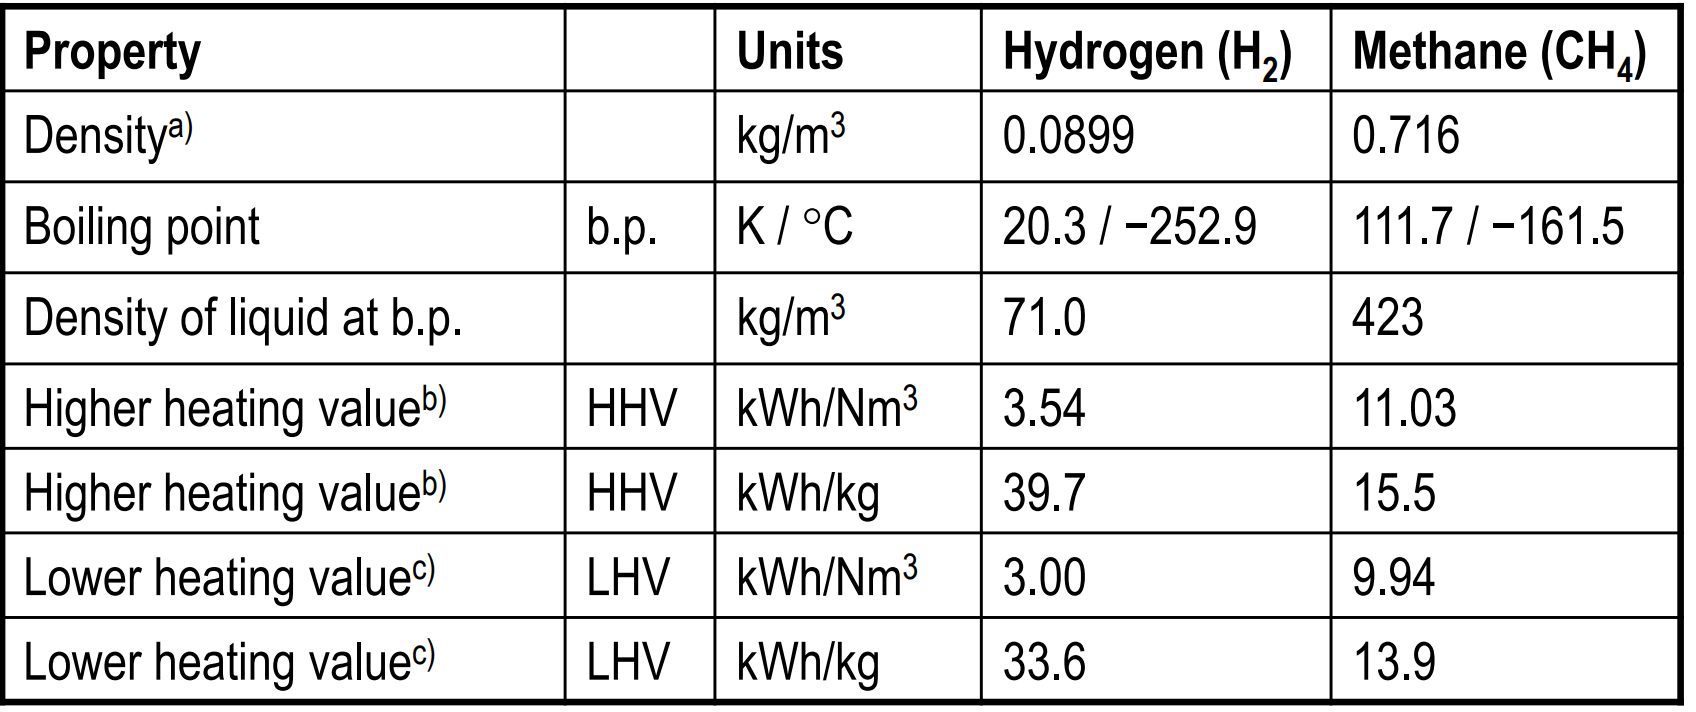
\includegraphics[width=1\linewidth]{src/hydrogen_table.png}
\end{figure}
% \vspace{-.8cm}
biggest consumers: ammonia production, petroleum refining, methanol production, (chemicals, metals, ...) \\
today: most $\mathrm{H_2}$ produced from fossil fuels, only 4\% electrolysis, $<$1\% renewable. \\

\subsection{production}
\vspace{-.5cm}
\begin{figure}[H]
    \centering
    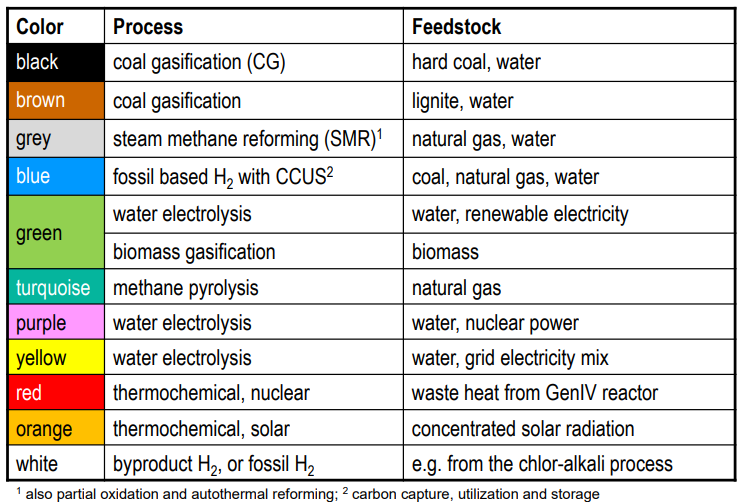
\includegraphics[width=1\linewidth]{src/H2_colors.png}
\end{figure}
% \vspace{-.5cm}
% \begin{tabular}{|>{\columncolor{black}\color{white}}p{1cm}|p{3.5cm}|p{3.5cm}|}
% \hline
% \textbf{Color} & \textbf{Process} & \textbf{Feedstock} \\ \hline
% \cellcolor{black}\color{white} black & coal gasification (CG) & hard coal, water \\ \hline
% \cellcolor{brown}\color{black} brown & coal gasification & lignite, water \\ \hline
% \cellcolor{gray} grey & steam methane reforming (SMR)\textsuperscript{1} & natural gas, water \\ \hline
% \cellcolor{blue} blue & fossil based H\textsubscript{2} with CCUS\textsuperscript{2} & coal, natural gas, water \\ \hline
% \cellcolor{green} green & water electrolysis & water, renewable electricity \\ \hline
% \cellcolor{lightgray} biomass & gasification & biomass \\ \hline
% \cellcolor{cyan} turquoise & methane pyrolysis & natural gas \\ \hline
% \cellcolor{purple} purple & water electrolysis & water, nuclear power \\ \hline
% \cellcolor{yellow} yellow & water electrolysis & water, grid electricity mix \\ \hline
% \cellcolor{red} red & thermochemical, nuclear & waste heat from GenIV reactor \\ \hline
% \cellcolor{orange} orange & thermochemical, solar & concentrated solar radiation \\ \hline
% \cellcolor{white}\color{black} white & byproduct H\textsubscript{2}, or fossil H\textsubscript{2} & e.g. from the chlor-alkali process \\ \hline
% \end{tabular}
\subsubsection{via Steam Reforming of Natural Gas (SMR)}
\begin{figure}[H]
    \centering
    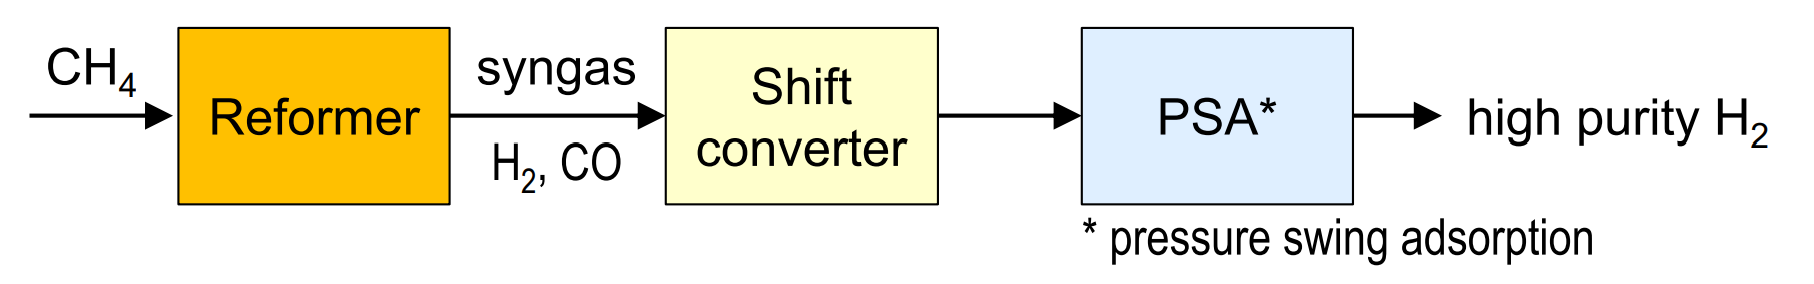
\includegraphics[width=1\linewidth]{src/PSA.png}
\end{figure}
\vspace{-1cm}
\begin{figure}[H]
    \centering
    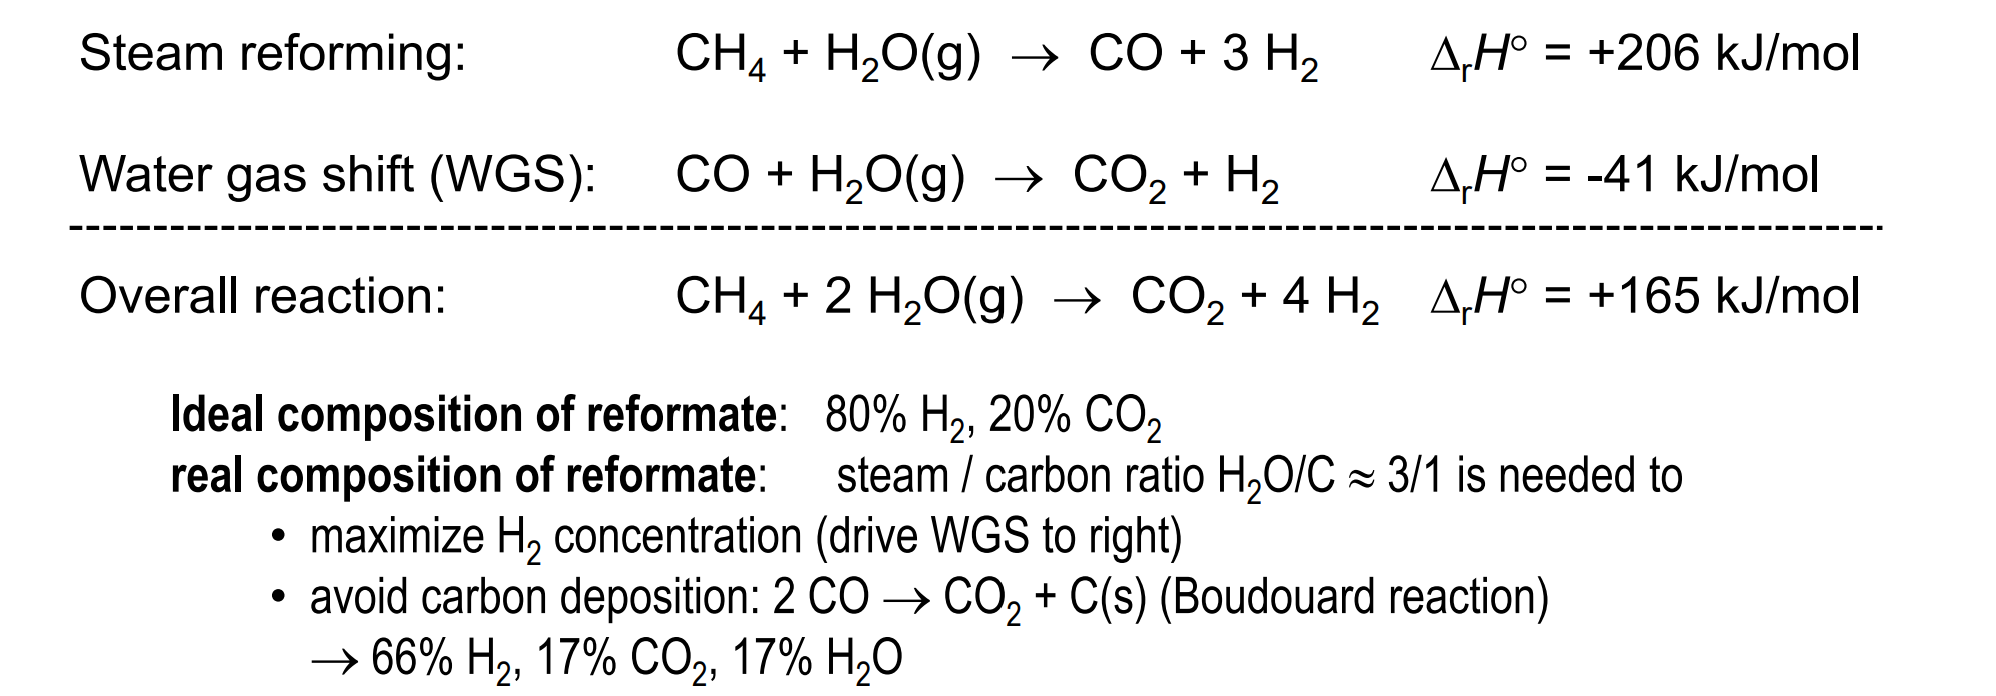
\includegraphics[width=1\linewidth]{src/h2_steam.png}
\end{figure}
steps:
\begin{enumerate}
    \item Natural gas (mainly methane, CH4) is catalytically decomposed in the presence of steam in a reactor at elevated
temperature (800-900°C) to CO and H2 (syngas)
    \item In the water gas shift (WGS) reactor (HT shift at ~500°C, LT shift at ~200°C), CO is converted to CO2 and
additional H2 is produced
\end{enumerate}
theoretical GHG: $\mathrm{\frac{m(CO_2)}{m(H_2)}=\frac{1mol\cdot 44\frac{g}{mol}}{4mol\cdot 2\frac{g}{mol}}}=5.5 \mathrm{\frac{kg_{CO_2}}{kg_{H_2}}}$

\subsubsection{from non-fossils}
- Water electrolysis using RE or nuclear power. \\
- Thermochemical water splitting, for example using the sulfur-iodine cycle, using high-grade heat (800°C) from a Gen IV nuclear reactor or concentrated solar radiation. \\
- Biomass gasification and purification 

\subsubsection{carbon footpring}
\begin{figure}[H]
    \centering
    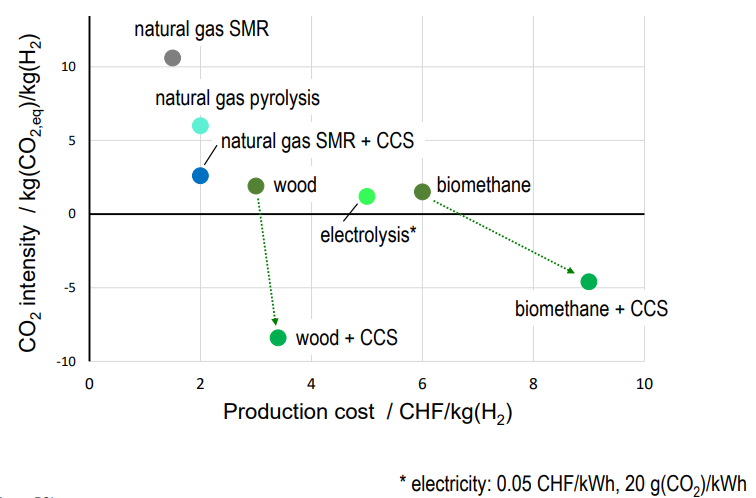
\includegraphics[width=1\linewidth]{src/h2_prod_GHG.png}
\end{figure}

\subsubsection{coal gasification}
similar to gas, just with gasification reactor, then WGS and PSA
% \subsubsection{cost}
% cost range from 2 CHF (natural gas), 5 CHF (electrolysis) to 9 CHF (biomehane + CCS) per kg of $H_2$. this is arther expensive for the yield of energy

%
\subsection{Distribution}
\textbf{Compressed gas (GH2)} \\
• mature technology
• low storage density
• reasonable for short range transport ($<$100 km)  \\
\textbf{liquid hydrogen (LH2)} \\
• $-253^\circ $ C
• liquefaction uses 30\% of energy content of H2
• mature technology \\
\textbf{solid inorganic hydrogen carrier (SIHC)} \\
• powder, e.g. NaBH4, easy to transport
• conversion losses
• carrier needs to be shipped back
• low technology readiness level \\
\textbf{methanol} \\
• widely used chemical, carbon-based energy carrier, 100 kg(H2)/m3
• H2 obtained through reforming (releases CO2) (similar to SMR, but lower temp.)
• toxic, but not carcinogenic or mutagenic, biodegradable \\
\textbf{ammonia} \\
b.p. -33.6C at 1 bar, 120 kg(H2)/m3
• established use as refrigerant and chemical feedstock (Haber-Bosch process !)
• shipping: fully refrigerated (-50C, ambient press.), semi-refrigerated (0C, 3-5 bar),
pressurized (20-25C, 16-18 bar)
• toxic and corrosive
• synthesis and cracking consume ~7-18\% of the H2 energy content \\
\textbf{liquid organic $H_2$ carrier} \\
• e.g. methylcyclohexane $\leftrightarrow$ toluene + 3 H2
• loss of up to 40\% of energy content for round-trip process
• carrier needs to be shipped back for ‘reloading’
• sometimes advertised as a ‘new thing’ but it is not* (like many other things…) 
% \begin{figure}[H]
%     \centering
%     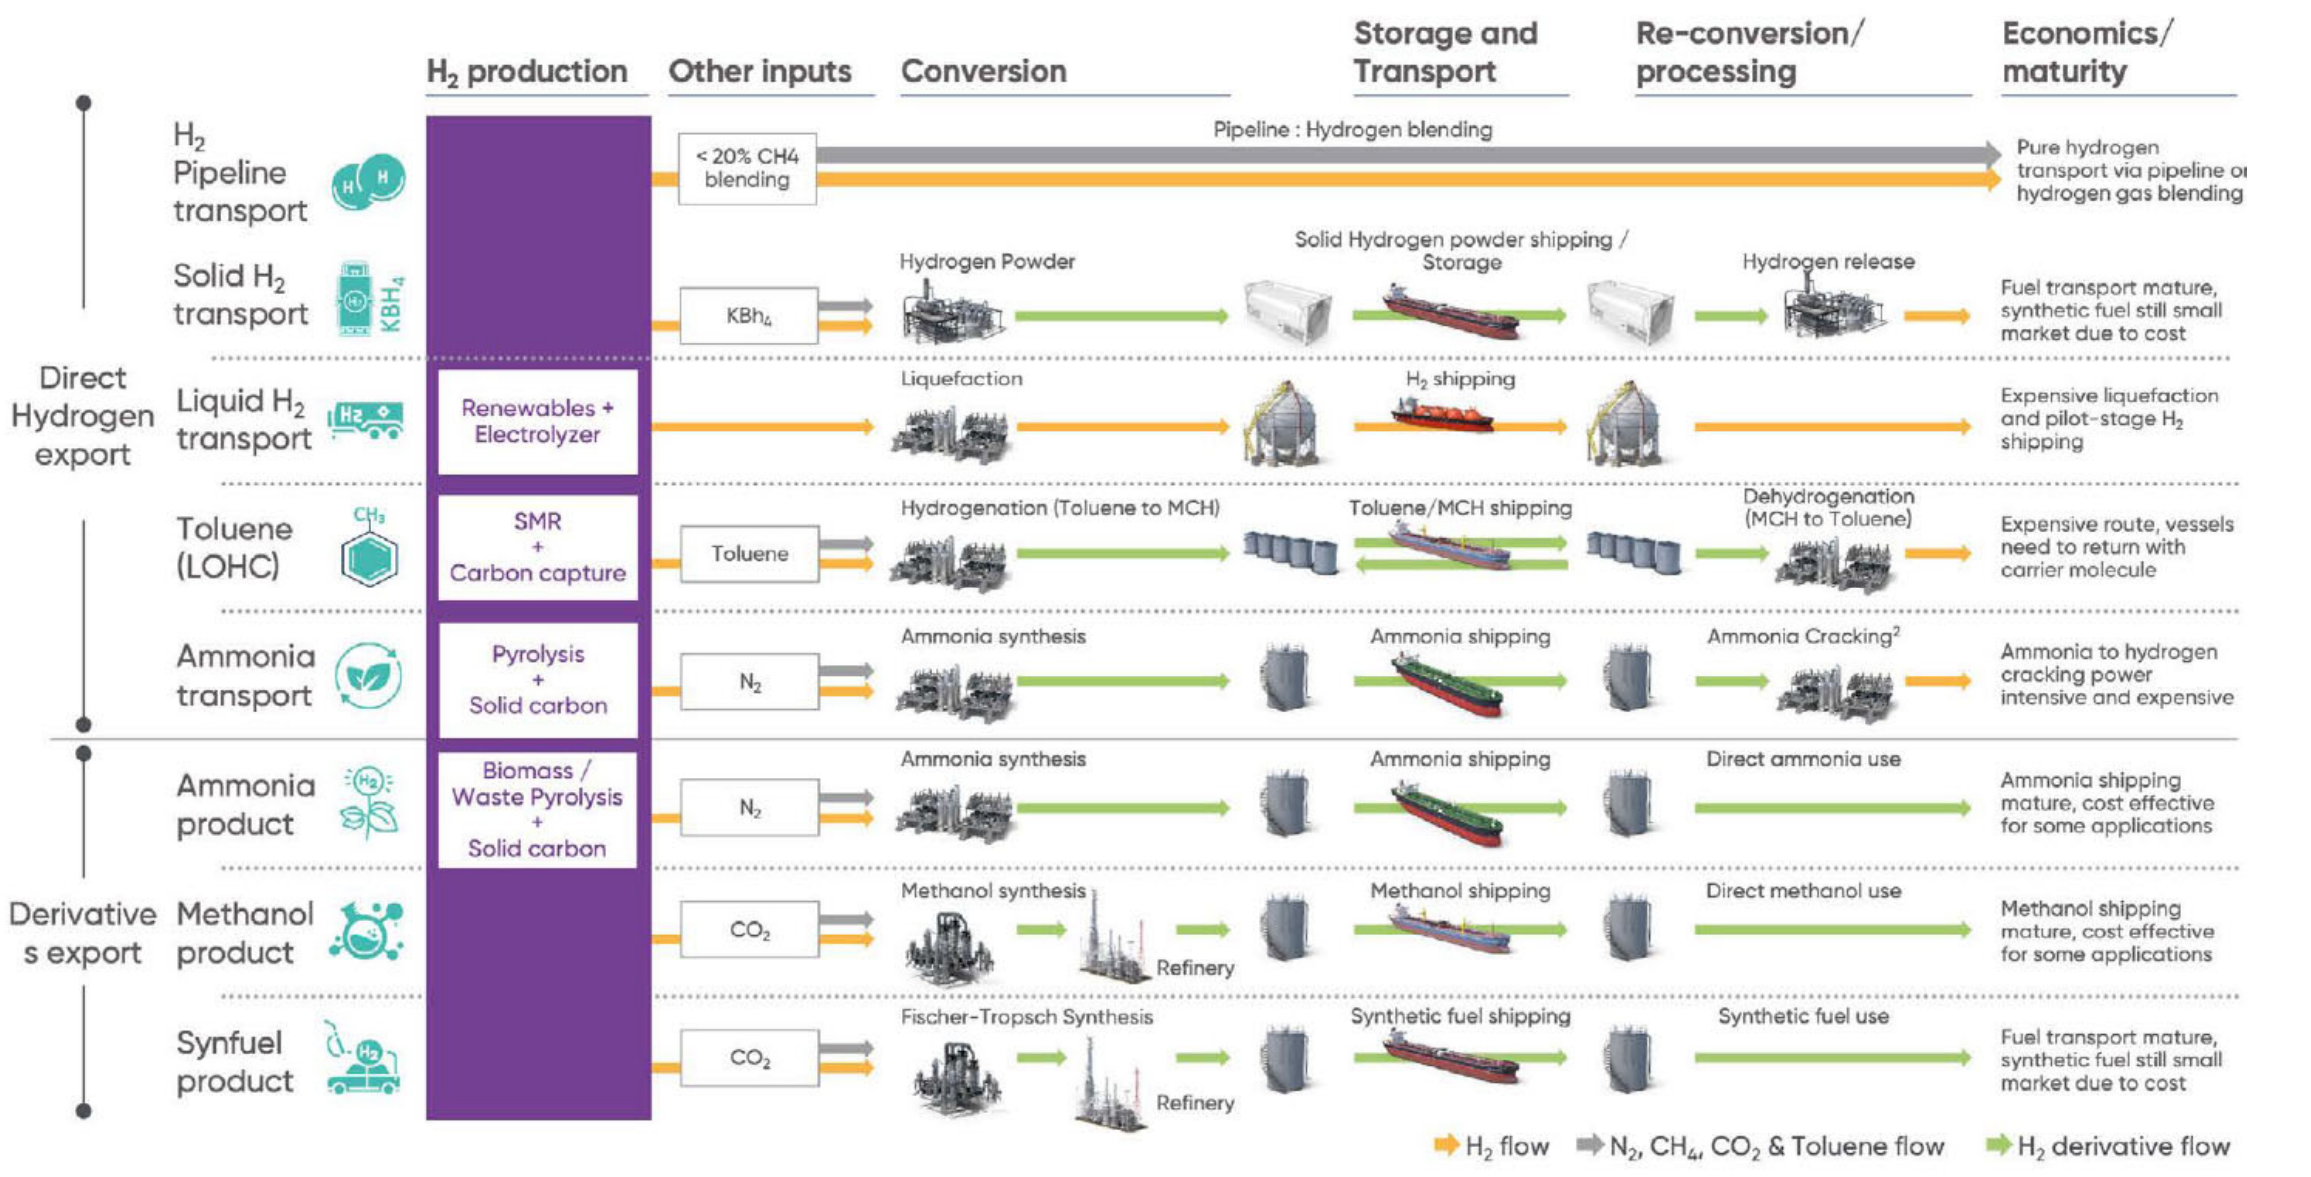
\includegraphics[width=1\linewidth]{src/h2_dist.png}
% \end{figure}

\subsection{Storage}
\begin{figure}[H]
    \centering
    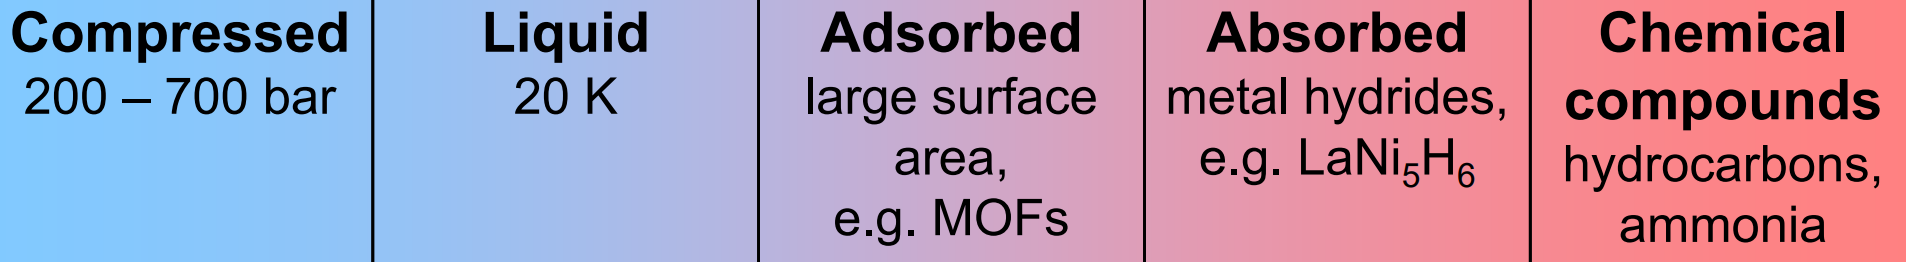
\includegraphics[width=1\linewidth]{src/h2_storage.png}
\end{figure}
from physical (left) to chemical (right) storage. \\
ideal gas law's:
$$pV=nRT=\frac{m}{M}RT$$
$$W_{1->2}=RT\cdot \ln{\frac{p_2}{p_1}}\text{ [kJ/mol]}$$ 
with p in $\mathrm{Pa}$, $M=2\mathrm{\frac{g}{mol}}$ \\
real gas law:
$$pV=Z\cdot nRT$$ 
with $Z_\mathrm{H_2}\approx1.45$ the compressibility factor

\subsubsection{conversions}
$\frac{\mathrm{Pa}}{\mathrm{bar}}=10^{-5} \quad\quad \mathrm{\frac{kJ}{kWh}}=3600$

\subsubsection{Local gas storage}
since LHV of gas $\approx 3\cdot$ LHV of $H_2$ we need 3 times more space.

\subsubsection{underground}
Oil and gas containing porous caverns \\
+ existing reservoir, leak tightness established \\
– limited local availability \\
– contamination with residual gas and extraction additives \\
Aquifers \\
+ abundant \\
– exploration required, ensure low leak rate \\
– fouling with microorganisms \\
– pressure given by hydrostatic pressure \\
Rock salt caverns \\ 
+ high purity, large volumes \\
– saturation with water vapor \\
total storage potential in Europe: 2’596 MtH2 (84.8 PWh)

\subsection{Prospects of $H_2$}
\begin{itemize}
    \item sustainable energy vector
    \item combustion not harmful
    \item seasonal storage possible
    \item sector coupling
\end{itemize}
\subsection{Issues of $H_2$}
\begin{itemize}
    \item very expensive still (unfavourable economics)
    \item only non-fossil $H_2$ makes sense
    \item storage/transport hard task
    \item efficiency drops (conversion, transport, cumbstion, ...)
\end{itemize}
\section{Fuel Cells}
\textbf{High \textit{T}}: \textit{T} needed for electrolyte conductivity \\
\textbf{Low/mid \textit{T}}: \textit{T} dictated by need of $H_2O$ for conductivity
\vspace{-.5cm}
\begin{figure}[H]
    \centering
    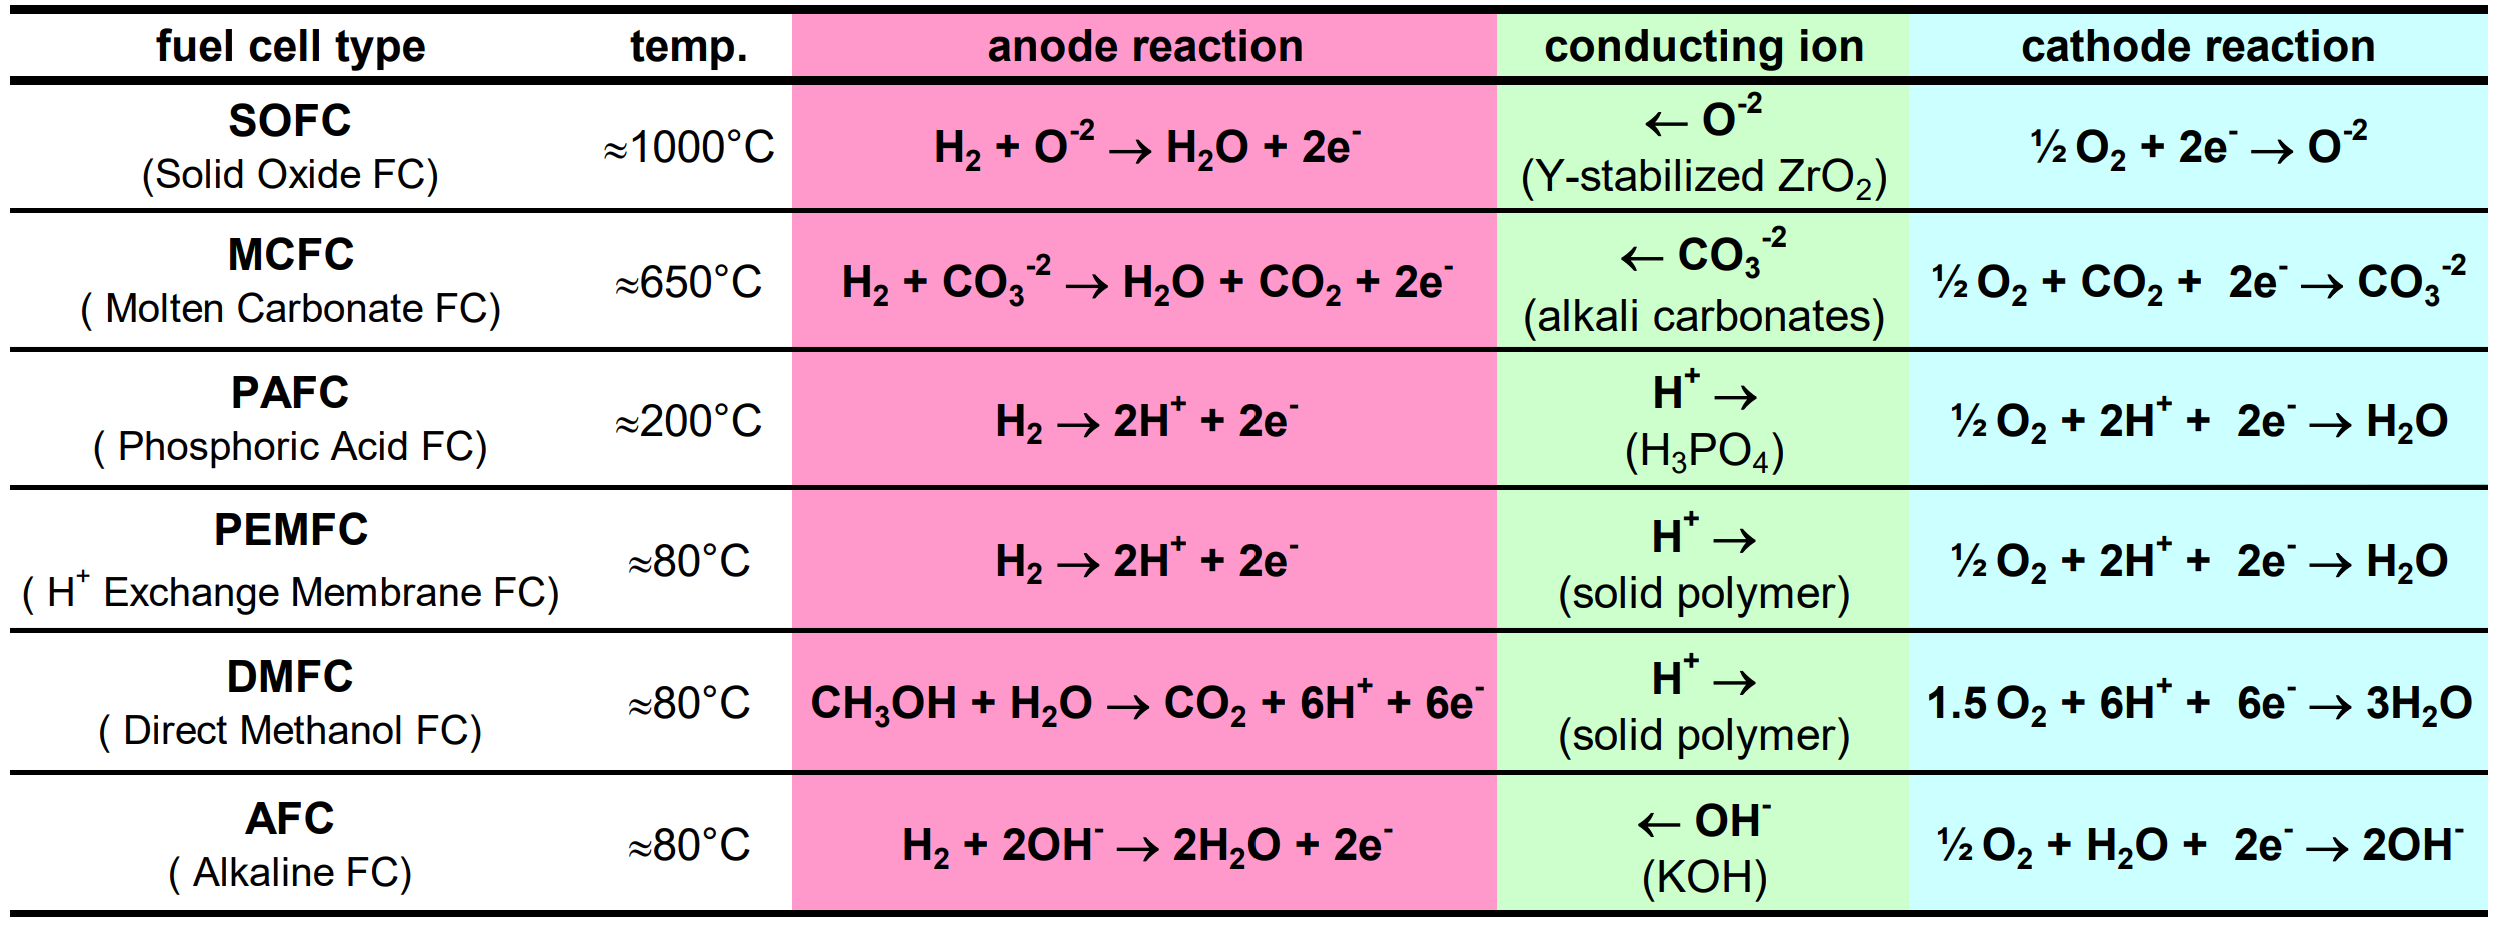
\includegraphics[width=1\linewidth]{src/fuel_cell.png}
\end{figure}
\vspace{-.5cm}
\subsection{Proton exchange membrane fuel cell (PEMFC)}
a.k.a. polymer electrolyte fuel cell (PEFC) \\
- Electrodes consist of porous composites of catalyst and $H^+$ -conducting polymer \\
- Electrolyte is solid, $H^+$-conducting polymer membrane (PEM) \\
% \item operation at $\approx 20-90^\circ C$ \\
- $\approx 1 \frac{W}{cm^2}$ 50-60\% efficiency \\
- applications: portable (automotive), residential \\
- issues: cost, durability
\subsection{Phosphoric acid fuel cell (PAFC)}
- Electrolyte is concentrated phosphoric acid imbibed in SiC \\
- $\approx$ 0.2-0.4 W/cm2, $\approx$60\% efficiency \\
- Applications: stationary \\
- Issues: cost, liquid electrolyte
\subsection{Direct methanol fuel cell (DMFC)}
- Similar electrodes and PEM electrolyte as in PEMFC \\
- $\approx$ 0.05-0.15 W/cm2, $\approx$ 20-30\% efficiency \\
- Applications: portable \\
-  Issues: cost, low efficiency, CH3OH-crossover
\subsection{Alkaline fuel cell (AFC)}
- Electrolyte is a 30-85\% KOH \\
- 0.2-0.5 W/cm2, $\approx$ 60\% efficiency \\
- Applications: spacecrafts, submarines
\subsection{Solid oxide fuel cell (SOFC)}
- Electrodes consist of porous composites: Ni @ anode, perovskite oxide @ cathode \\
- Electrolyte is a O2- conducting ceramicmaterial (ZrO2-Y2O3) \\
-  $\approx$ 0.2-0.3 W/cm2, $\approx$ 60\% efficiency \\
- Issues: thermal cycling
\subsection{Molten carbonates fuel cell (MCFC)}
- Electrodes consist of porous composites:
Ni @ anode, Li-Ni oxide @ cathode \\
- Electrolyte is a CO32- -conducting fused salt \\
- $\approx$ 0.08-0.15 W/cm2, $\approx$ 55\% efficiency \\
- Issues: durability, NiO-reduction @ cathode

\subsection{Thermodynamic FC efficiency}
Thermodynamic FC efficiency, usually based on HHV:
$$\epsilon_{th} = \frac{E_{rev}}{E_{th(HHV)}}\approx 83\%$$
but LHV also used for comparison between tech.
\begin{align*}
    E_{\text {rev }}=1.23-0.9 \cdot 10^{-3}(T-298)+\frac{2.303 R T}{2 F} \\
    \cdot\log \left(\frac{\left(p_{H 2} / p_{H 2}^*\right)\left(p_{O 2} / p_{O 2}^*\right)^{0.5}}{(R H / 100)}\right)
\end{align*}
where $x^*$ is the standard concentration $p_{tot}-p_\mathrm{H_2O}$ \\
or if given $E_{rev}=-\frac{\Delta G}{zF}=-\frac{\Delta H-T\Delta S}{zF}$
overall FC efficiecny then is
$$\epsilon_{FC}=\epsilon_{voltage}\cdot \epsilon_{th(HHV)}= \frac{E_{cell}}{1.48 V}$$

\subsubsection{partial pressure law}
$$
x_{\mathrm{i}}=\frac{p_{\mathrm{i}}}{p}=\frac{n_{\mathrm{i}}}{n}
$$
with $p_i,  n_i$ the partial pressure / moles of species $i$ respectively \\
$p,n$ the total pressure / \# moles respectively

\subsubsection{example: $\mathrm{O_2}$ and air FC}
FC operating with $\mathrm{H_2,O_2},T=80^\circ C, p_{tot}=150\mathrm{kPa_{abs}}, RH=100\%, p^{sat}_\mathrm{H_2O}(80^\circ C)=50\mathrm{kPa}$: \\
$p_\mathrm{H_2O} = p^{sat}_\mathrm{H_2O}\cdot RH=50\mathrm{kPa}$ \\
$p_\mathrm{H_2}=p_\mathrm{O_2}=p_{tot}-p_\mathrm{H_2O}=100 \mathrm{kPa}$ \\
$E_{rev}=\dots=1.181 \mathrm{V}$ \\
if cathod is air-fed instead of $\mathrm{O_2}: p_\mathrm{O_2}'=0.21\cdot p_\mathrm{O_2}$ \\
thus $E_{rev}'=\dots=1.169 \mathrm{V}$

\subsection{example: $E_{cell}$}
If the sum of reversible potential and kinetic overpotential at that current is 0.75 V and the mass transport overpotential is negligible, what is the operative potential considering ohmic losses of $33$ mV? \\
$E_{\text {cell }} =\Delta E_{\text {rev }}+\eta_{mtx}+\eta_R+\eta_{\text {kin }}=0.75 + 0 - 0.033=0.717 \mathrm{V}$

\subsubsection{power density}
$P=V_{operative}\cdot i \quad\left[\mathrm{\frac{W}{cm^2}}\right]$


\section{Electrolysis}
electrolyzers are a sort of electrolysis cell \\
anode (OER): $\mathrm{H_2O\rightarrow \frac{1}{2}O_2+2H^+ + 2e^-}$ \\
cathode (HER): $2H^+ + 2e^- \rightarrow H_2$
\subsection{IV curve}
\begin{figure}[H]
    \centering
    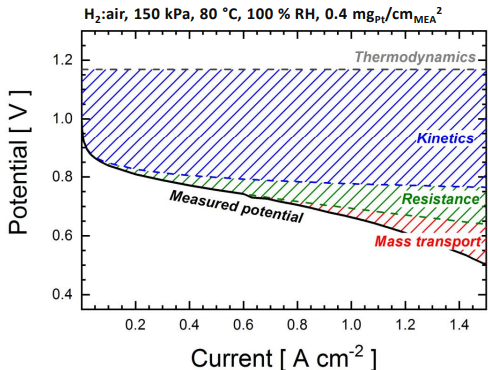
\includegraphics[width=1\linewidth]{src/electrolysis_iv.png}
\end{figure}
with the following main parameters
\subsubsection{overpotential effects}
$$
\begin{aligned}
E_{\text {cell }} & =\Delta E_{\text {rev }}+\eta_{mtx}^{\text {positive }}+\eta_R^{\text {positive }}+\eta_{\text {kin }}^{\text {positive }} \\
& -\left(\boldsymbol{\eta}_{\boldsymbol{m t x}}^{\text {negative }}+\eta_R^{\text {negative }}+\eta_{\text {kin }}^{\text {negative }}\right)
\end{aligned}
$$
Sluggish oxygen-evolution-reaction effects ($\eta_{OER}$) is main source of performance losses. Ohmic losses, small transport limitations also relevant.
\subsubsection{electrolyzer efficiency}
$\epsilon_{EL}=\frac{\Delta_r H^0}{zFE_{cell}}\quad$
LHV: $\epsilon=\frac{1.25}{E_{cell}}\quad$     HHV: $\epsilon=\frac{1.48}{E_{cell}}$
\subsubsection{H2 crossover}
Concentration gradients drive permeation of H2 from anode to cathode and of O2 from cathode to anode. \\
PROBLEM: lower explosion limit for H2 in O2 is $\approx$ 4\%, so H2 concentration in O2 (i.e., at anode) should remain $\leq$ 2\% \\
Particularly relevant at low currents

\subsubsection{energy}
$W=Q\cdot E_{cell}=z\cdot F\cdot n\cdot E_{cell}=z\cdot F\frac{pV}{RT} E_{cell} \quad[\mathrm{kJ}]$
$$W_e = zFE_{cell} \quad \left[\mathrm{\frac{kJ}{mol}}\right]$$
% $W=z\cdot F\cdot n\cdot E_{cell}=z\cdot F\frac{p\cdot V}{R\cdot T}E_{cell}$\\
V-specific energy consumption:
$$W_V=z\cdot F\cdot E_{cell}\frac{p}{R\cdot T}=W_e\frac{p}{RT} \quad\left[\mathrm{\frac{kJ}{m^3}}\right]$$
mass-specific energy consumption:
$$W_m=z\cdot F\frac{E_{cell}}{M(H_2)}=\frac{W_e}{M_\mathrm{H_2}} \quad\left[\mathrm{\frac{kJ}{kg}}\right]$$

\subsection{high $T$: solid oxide electrolysis cell (SOEC)}
- reaction basically inverse of PEMFC \\
- operation 500-850C \\
- $80-90\%$ efficiency \\
- issues: thermal cycling
\subsection{Low $T$: alkaline \& proton exchange electrolyzers}
- alkaline: inexpsnive but low currents and pressure
- proton-conducting membrane: high currents and pressure but costly and scarce materials
\subsection{example: EL stack}
Stack of 400 in series cell, 100kg $\mathrm{H_2}$/day, active area of 500cm$^2$, what is the avg. current density? \\
$\Dot{n}_\mathrm{H_2} = \frac{\Dot{m}_\mathrm{H_2}}{M_\mathrm{H_2}}= \frac{100\mathrm{kg}}{2\cdot10^{-3}\mathrm{\frac{kg}{mol}}}\cdot\frac{1}{\Delta t}=0.578\mathrm{\frac{mol}{s}}$ \\
$i=\frac{I}{A}=\frac{\Dot{n}_\mathrm{H_2}\cdot z\cdot F}{N_{cells}}/A=\frac{279 \mathrm{A}}{500 \mathrm{cm}^2}$

\subsection{example: water splitting}
calc. rev. potential of water splitting at $25^\circ\mathrm{C}, p_{gas}=200\mathrm{bar}$: \\
$$E_{rev}=E^0_{rev}-\frac{RT}{zF}\ln{\left(\frac{a_\mathrm{H_2}\cdot \sqrt{a_\mathrm{O_2}}}{a_\mathrm{H_2O}}\right)}=-1.23-\dots=-1.3234\mathrm{V}$$
with $p_\mathrm{H_2}=p_\mathrm{O_2}=200$ bar, $p_\mathrm{H_2O}=1$ bar.

\section{Batteries}
\subsection{Theoretical and Practical Capacity of Cell}
for general reaction $aA+bB\leftrightarrow cC+dD$:
$$Q_{spec,th,cell}=\frac{z\cdot F}{3.6\mathrm{\frac{A\cdot s}{mA\cdot h}}\left(a M_{w,A}+b M_{w,B}\right)}  \quad\left[\mathrm{\frac{mAh}{g}}\right]$$
the practical capacity will be lower due to inactive components/inefficiencies.

\subsubsection{Gravimetric energy density}
$E_{g}=U\cdot Q_{spec}\quad \left[\mathrm{\frac{Wh}{kg}}\right]$

\subsection{General}
\textbf{cell}: device capable of generating electrical energy from chem. reactions or using elec. energy to cause chem. reactions \\
\textbf{battery}: multiple cells + external \\ connections via string: add voltages or in parallel: add currents \\
xSyP: x cells serial, y parallel (total x*y)
\subsection{coin cell}
Small size, easy to stack
- Mainly reserved as primary
batteries in watches, gauges
- Rechargeable button cells
do not allow fast charging
- Limited new developments 
\subsection{cylindrical cell}
- Mainly reserved as primary batteries in watches, gauges \\
- Rechargeable button cells do not allow fast charging \\
- Classic packaging for primary \& secondary cells \\
- Holds internal pressure without deforming case
\subsection{prismatic cell}
- best use of space \\
- allows flexible design \\
- higher cost \\
- less efficient thermal management \\
- shorter life
\subsection{pouch cell}
- light and cost-effective \\
- simple, flexible, lightweight \\
- but: humidity exposure, hot temp's shorten life \\
- design must include allowance for 8-10\%
\subsection{materials}
\textbf{for positive electrodes} \\
- LCO, LMO, LFP, NCA, LR-NCM \\
\textbf{for negative electrodes} \\
- Graphite, LTO, Silicon, Tin

\subsection{new batteries tech.}
\textbf{Li-metal} \\
charge, anode: $\mathrm{Li^+ + e^-\rightarrow Li}$ \\
+ Higher energy density  \\
- but Li dendrites can form \\
\textbf{Solid-state battery} \\
+ safety and potentially higher energy\\
- but interface stability poor \\
\textbf{Na-ion batteries} \\
+ abundance, no critical materials\\
- but lower energy density

\subsection{examples}
\textit{How many lithium ions can be extracted per formula unit, if the practical capacity is 260 Ah/kg?} \\
$n_\mathrm{Li}=z=Q\cdot3.6\frac{M_w}{F} = 1.13$ \\
\textit{Calculate the theoretical capacity of Li2MnO3.} \\
$\mathrm{Li_2MnO_3 \leftrightarrow 2Li^+ + 2e^- + MnO_3}$ \\
$Q_{spec}=\frac{z\cdot F}{3.6\cdot M_\mathrm{Li_2MnO_3}}=458.9 \left[\mathrm{\frac{Ah}{kg}}\right]$

\section{Electric Mobility}
\subsection{E-mobility readiness}
determined by \\
- The year in which efforts began \\
- Average income of population \\
- Government incentives \\
- Orchestrated buildup of charging infrastructure \\
- Electromobility image (public perception) \\
\textbf{limitations:} \\
- Technolgical: Limiting driving range \\
- Environmental: environmental impact of battery production \\
- Financial: price of new electric car \\
- Infrastructure: Insufficient amount of public charging stations \\
\textbf{future electrified transport types:} \\
- heavy trucks, large ships, long haul ships, large airplanes, trains \\
\textit{GEMRIX}
Global Electric Mobility Readiness Index. \\
Factors: Macroeconomic, EV market \& competitive landsacpe, customer EV readiness, charging infrastructure, TCO and regulation. \\
Best countries: Norway, China, Germany, Singapore UK. \\
Norway is an extreme case, selling 86\% of BEV of new vehicles. \\
Bad rating: Low income/industrializing countries. \\
\subsection{Types of EVs}
\textbf{Hybrids (HEVs)} exclusively rely on regenerative braking, may allow exclusively electric driving. \\
\textbf{Plug-in hybrids (PHEVs)} can be connected to grid, typically allow $<$ 80 km electric driving. \\
\textbf{Battery and Fuel cell electric vehicles (BEVs, FCEVs)} can be regarded as fully electric. \\
FCEVs to be fueled with (electro)chemically produced H2.
\subsection{efficiency}
round trip efficiency of tech's: \\
BEVs: 77\% vs. 33\% Hydrogen vs. 23\% Powert-to-liquid vs. 22\% power-to-methane.
\subsection{charging}
from AC chargers (22 kW) to DC chargers (50 kW) to ultra-fast charging ($>$150 kW).
\subsection{sectors}
the electrification in many sectors such as ships, trucks and plains will depend on higher energy density batteries and/or higher efficient fuell cells.

\section{Flow batteries}
motivation:  \\
1. different grid-scale energy storage applications from short term (less 2h) to long term (weeks, months) \\
2. Flow batteries specifically designed for stationary storage: independent energy and power rating, long cycle life
\subsection{broad architecture}
- active material stored externally \\
- non-reacting electrodes \\
- forced electrolyte flow \\
- rechargeable 
\subsection{Redox Flow batteries (RFBs)}
+ grid scale storage 10kWh - >100 MWh \\
+ Independent scalibility of energy and power \\
+ long cycle and design life, low self discharge \\
- low energy and power density \\
\begin{figure}[H]
    \centering
    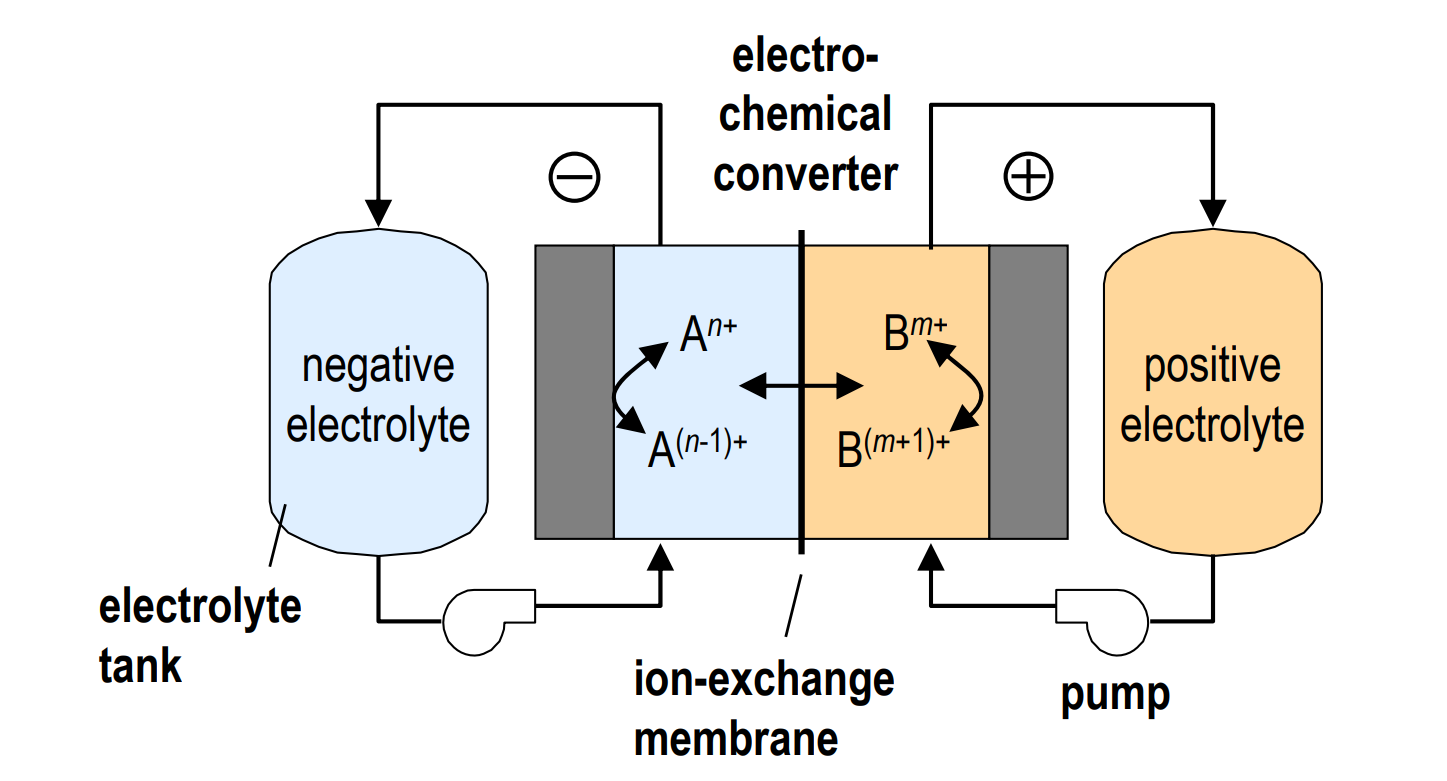
\includegraphics[width=0.75\linewidth]{src/RFB.png}
\end{figure}
\subsubsection{RFB types}
1. all-vanadium (high cost, most common) \\
2. $H_2/Br_2$ gas half-cell, rapid kinetics \\
3. $Fe/Cr$ cheap but $U_{cell}\approx 1V$ \\
4. $Zn/Br_2$ hybrid, low material cost \\
\begin{figure}[H]
    \centering
    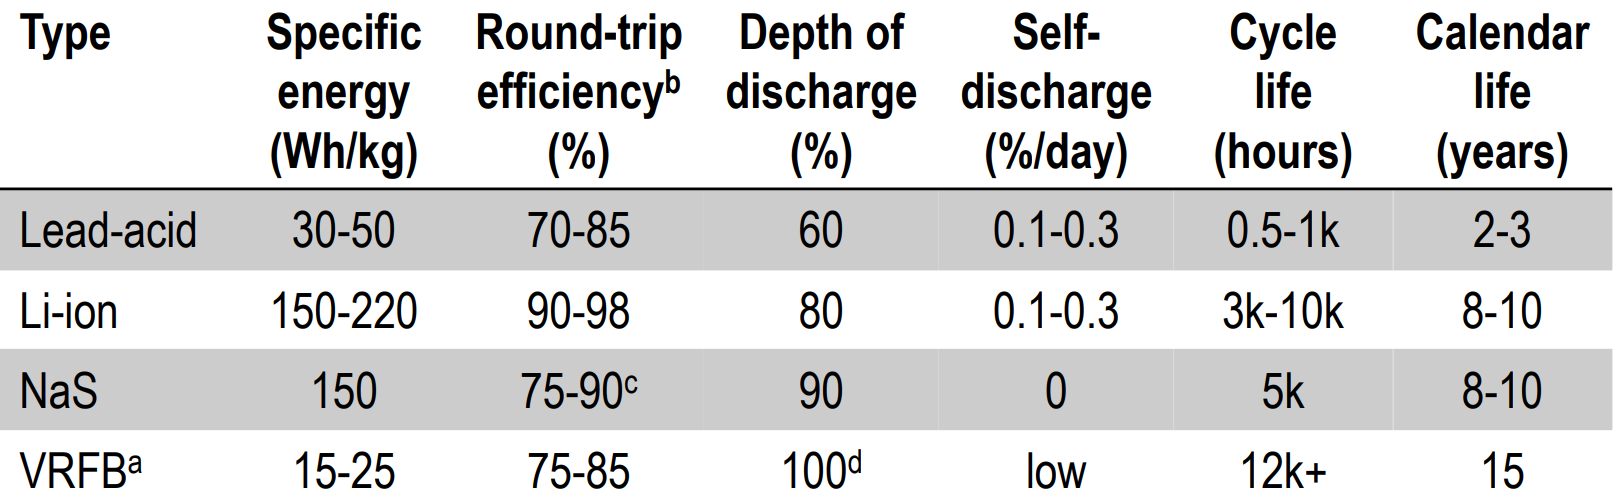
\includegraphics[width=1\linewidth]{src/RFB_comp.png}
\end{figure}
\subsection{VRFB}
neg. electrode: $V^{3+} + e^- \leftrightarrow V^{2+} \quad E^0=-.26V$ \\
pos. electrode: $VO_2^+ + 2H^+ + e^- \leftrightarrow VO^{2+} + H_2O \quad E^0=1V$ \\
contains vanadium-ions in different oxidation state on both sides

\subsubsection{membrane / separator}
must have high coulombic eff. $\epsilon_C$ to prevent crossover from redox-active species. This can be achieved by higher current densities since charge and discharge times get shorter which allows less self-discharge of vanadium. \\
high voltage eff. $\epsilon_V$ for low resistance / high mobility of electrolyte ions. this decrease with higher current density cause overpotentials increase with current density \\
thus there is a global max. of $\epsilon_C \cdot\epsilon_V$ \\
$\mathrm{SoC}=\frac{x^{2+}}{x^{2+}+x^{3+}}$
\subsection{Performance metrics}
current: $I=i\cdot A$ \\
efficiencies: $\epsilon_C=t_d/t_c$, $\epsilon_V=\overline{U}_d/\overline{U}_C$, $\epsilon_{tot}=\epsilon_C\cdot\epsilon_V$ \\
discharge capacity: $Q_d=I\cdot t_d$ \\
capacity utilization: $u_d=Q_d/Q_0$
\subsection{comparison to Li-ion}
- higher cost \\
- more complex balance-of-plant components \\
- relative low round-trip eff. $~70\%$ \\
+ but: uses other materials (maybe less scarce), longer storing time, few capacity fading
\subsection{nominal capacity}
$$Q_0=c\cdot z\cdot F\cdot V$$
with $Q_0$ the nominal capacity $c$ the concentration in $\left[\mathrm{\frac{mol}{L}}\right]$, $V$ the volume $[V]$, $F$ Faraday const. $26.8\left[\mathrm{\frac{Ah}{mol}}\right]$

\section{Super-capacitors}
- short term, fast, power devices, very high \# of cycles, diverse application space (buffering peaks, damping fluctuations in grid, storing braking energy)
\subsection{Definition}
Electronically double-layer capacitors (\textbf{EDLCs}) store electric energy in the elec-chem double layer (Helmholtz layer)
\subsection{Features}
% EDLCs are power devices with comparably low energy density, used in applications with short-charge discharge ‘bursts’ where a high number of cycles (can be millions) are accumulated
\begin{itemize}
    \item very high rates of charge and discharge
    \item little degradation
    \item good reversibility
    \item low toxicity of materials used
    \item high efficiency >$95\%$
    \item low energy density
\end{itemize}
\subsection{equations}
\begin{align*}
    &Q=C\cdot U=\int Idt & \\
    &W_e =\frac{1}{2}C\cdot U^2 &\Delta t=\frac{Q}{I}
\end{align*}

\subsection{technologies}
1. polymeric film, ceramic\\
2. metal oxide, electrolytic\\
3. Super-capacitor: electrochem. double layer\\
from left to right: 
\begin{figure}[H]
    \centering
    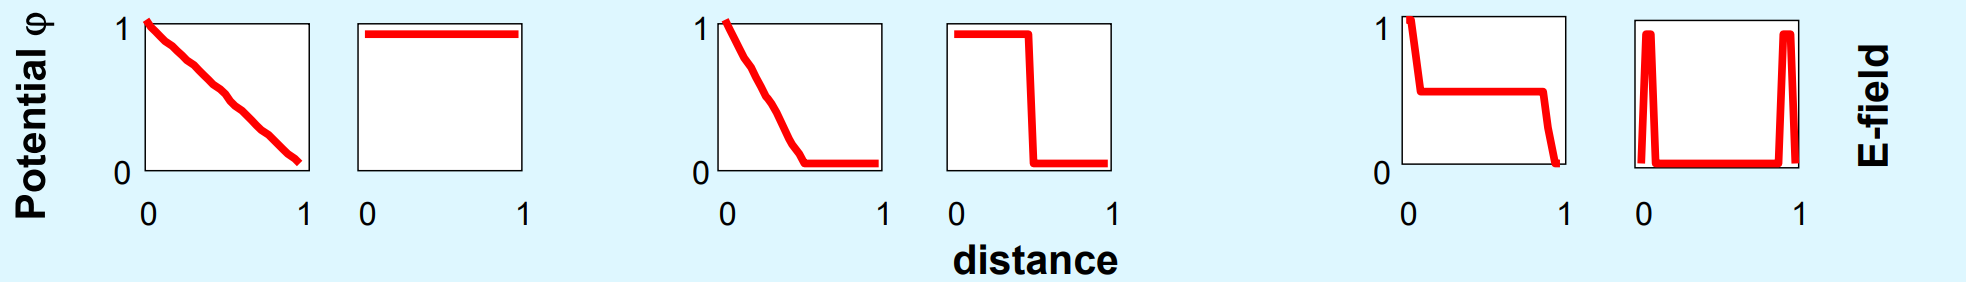
\includegraphics[width=1\linewidth]{src/supercap.png}
\end{figure}
\subsection{Electrochemical double layer (EDL)}
excess charge on electrode leads to formation of chmical double layer. thickness .5-2nm\\
The \textbf{Helmoholtz model} of the EDL assumes a linear drop of the potential in this layer (const. $\varphi$ within electrode and electrolyte). with this we can define the specific capacitance $C=\frac{\sigma}{\Delta \varphi}$. \\
Thus a simple equivalent circuit of an EDLC comprises 2 capacitors and one resistance (electrolyte): $C_{tot}=\frac{C}{2}$ \\
gravimetric capacitance of supercapacitor: $c_\mathrm{g,sc}=c_g/4$
with $c_g$ for 1 electrode \\
Thus we want to maximize inter facial area at the electrodes and max. operating voltage for low losses. For the capacitance:
$$C=\epsilon\epsilon_0\frac{A}{d}$$
\subsection{Cyclic Voltammetry}
method to determine capacitance of electrode
\begin{figure}[H]
    \centering
    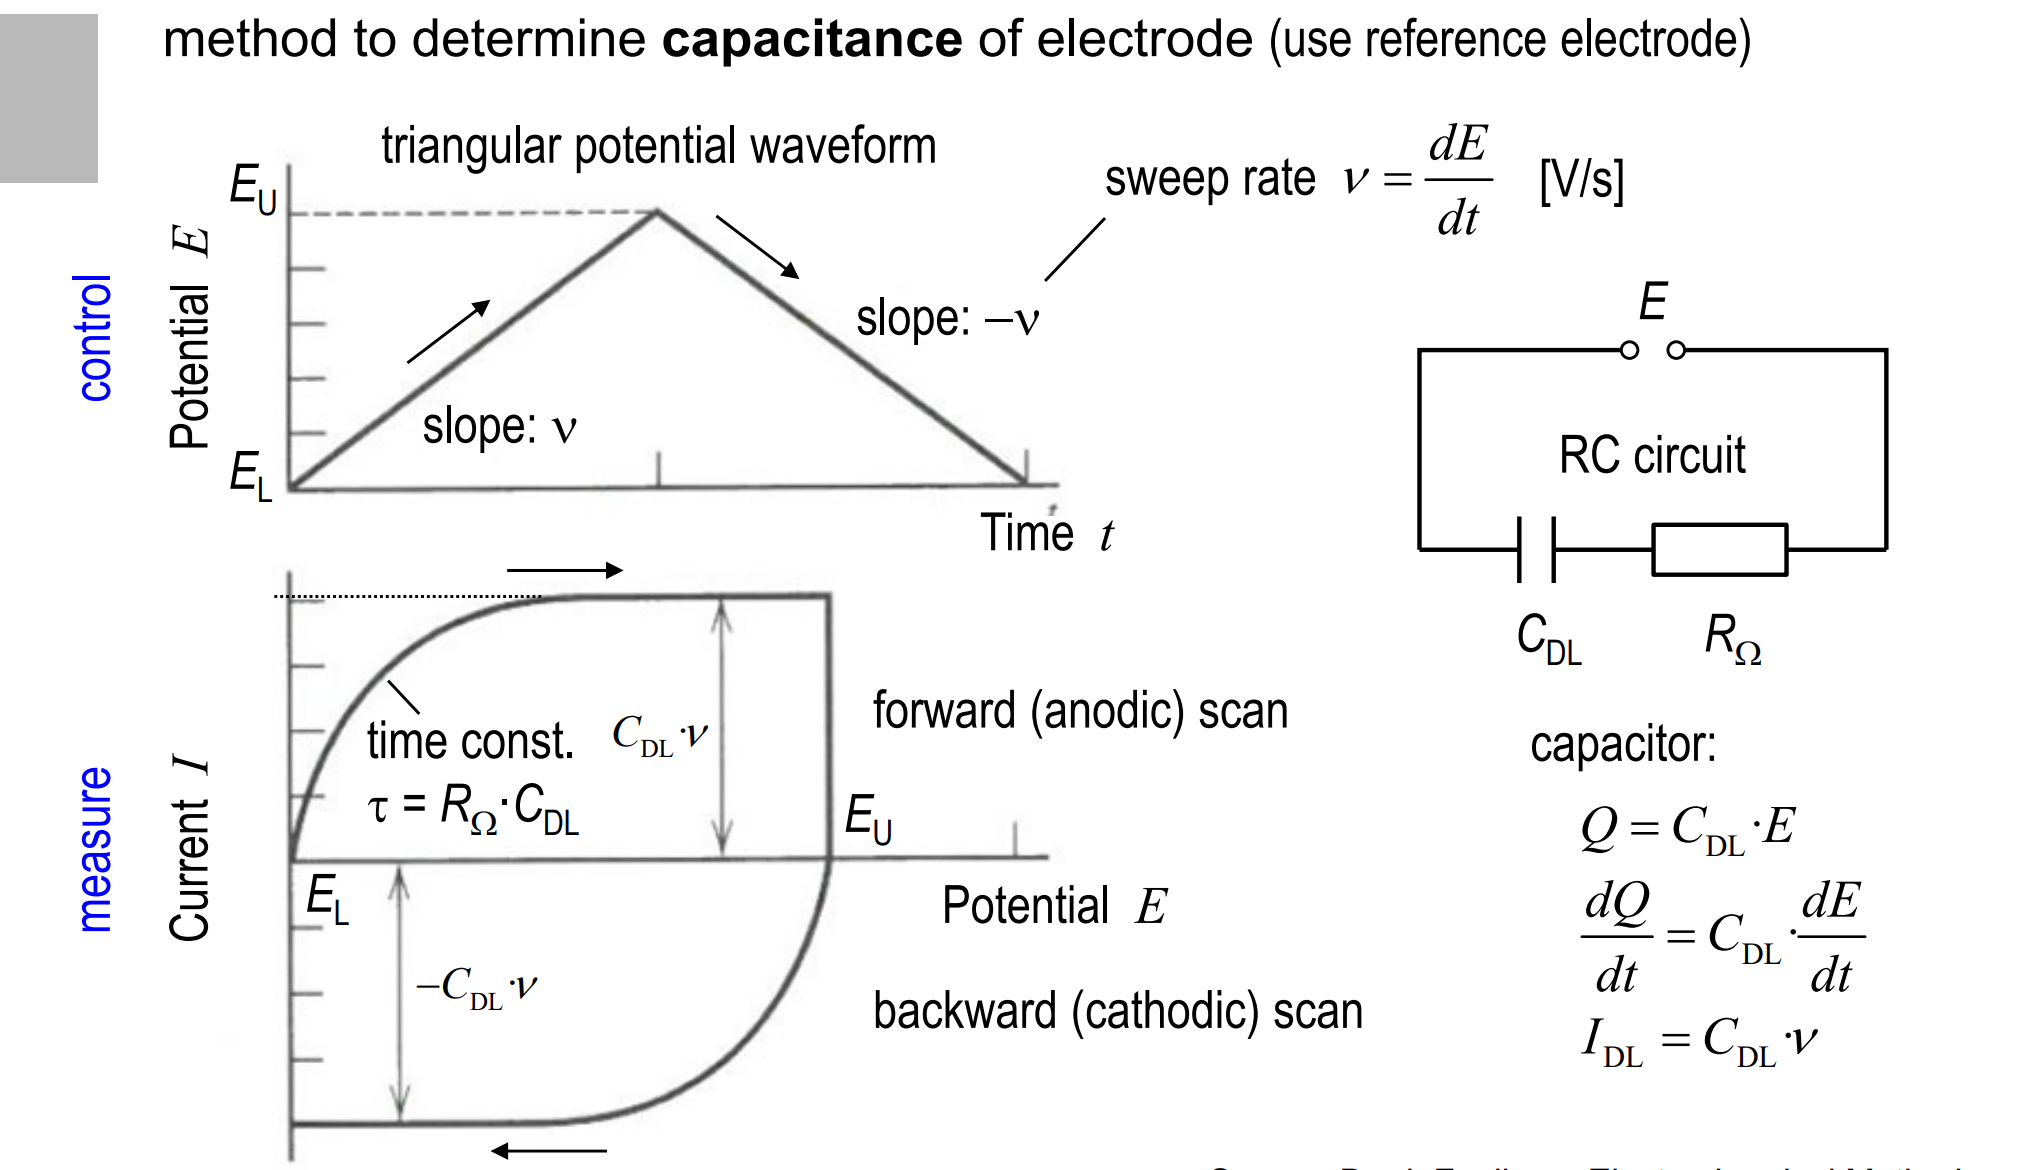
\includegraphics[width=0.75\linewidth]{src/cv.png}
\end{figure}

\subsection{components}
electrodes: microporous carbon \\
electrolyte: quaternary ammonium salt in propylene
carbonate (PC) or acetonitrile (ACN)

\subsection{characterization}
capacitance of cell: $I=\frac{dQ}{dt}=C_{SC}\frac{dU}{dt}$ \\
gravimetric capacitance: $c_{g,SC}=\frac{I}{v\cdot m_{sc}}$ with $v$ the sweep rate\\
gtav. cap. of electrode: $c_{g,e}=\frac{2C_{SC}}{m_{SC}/2}=4c_{g,SC}$

\subsection{ragone plot}
plots specific power to specific energy of various technologies

\subsection{discharge behaviour}
\subsubsection{constant current}
$$P(t)=U(t)\cdot I=(U_0-\Delta U -\alpha t)I$$
where $\Delta U$ is the voltage drop due to internal resistance
\subsubsection{constant power}
need to increase current as voltage decreases \\
\begin{figure}[H]
    \centering
    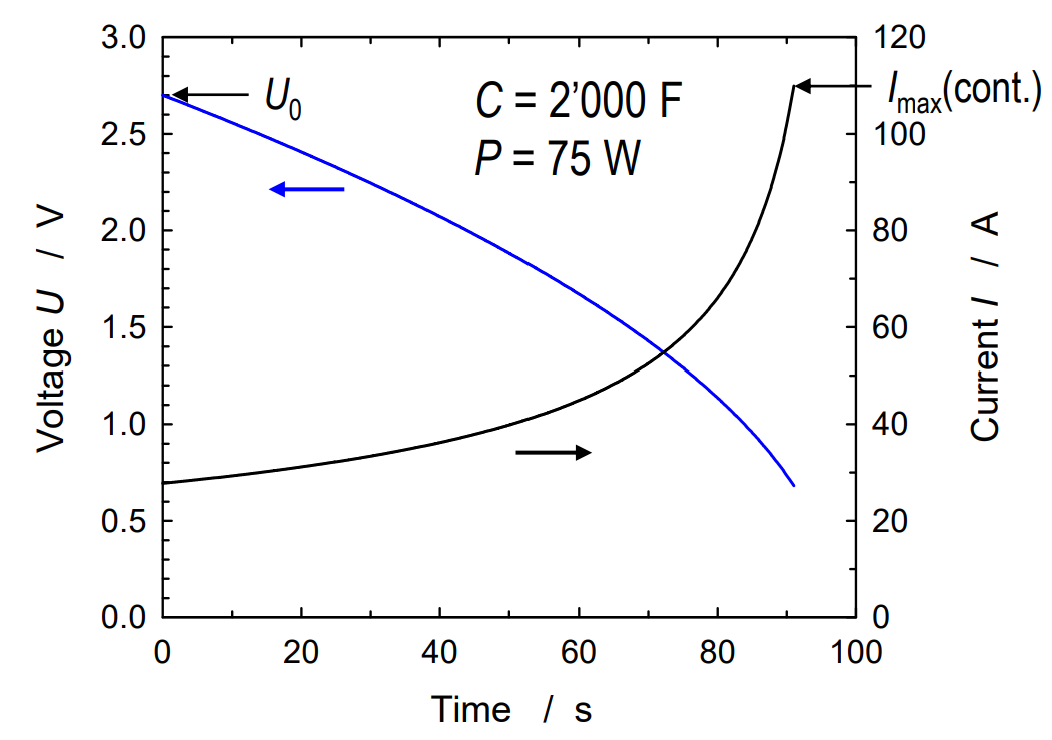
\includegraphics[width=0.5\linewidth]{src/const_power.png}
\end{figure}
neglecting internal resistance: \\
$P=U(t)I(t)=-U(t)\cdot C\cdot \frac{dU(t)}{dt}$ \\
$U(t)=\sqrt{U_0^2-2\frac{P}{C}t}$ and $SOC=Q/Q_0=U/U_0$
\subsection{maximum power density}
$p_{max}=\frac{U_{OCV}^2}{4R}$ with $U_{OCV}$ the open circuit voltage
\subsection{comaprison to battery}
\begin{tabular}{|p{4cm}|p{2cm}|p{2cm}|}
\hline
\textbf{Property} & \textbf{Li-Ion Battery} & \textbf{EDLC} \\ \hline
Time for charge / discharge & 0.3 .. 6 h & 0.3 .. 30 s \\ \hline
Voltage (V) & 3.6 .. 4.2 & 2.5 .. 2.8 \\ \hline
Specific energy (Wh/kg) & $>$ 170 & $<$ 6 \\ \hline
Specific power (W/kg) & $<$ 1'000 & $<$ 10'000 \\ \hline
Cycle lifetime (\# cycles) & 500 – 2'000 & 50k – 1M \\ \hline
Round-trip efficiency (\%) & 70 – 85 & 85 – 98 \\ \hline
Self discharge rate @ r.t. & 2 \% / month & 4 \% / month \\ \hline
Temperature range (°C) & -40..+80 & -40..+65 \\ \hline
Cost (\$/kW) & 200 & 8 \\ \hline
Cost (\$/kWh) & 500a & 12'000 \\ \hline
State of charge determination & difficult & very simple \\ \hline
\end{tabular}

\subsection{application}
\textit{in grid scale storage:} stabilize output of solar and wind power, ensuring smooth power ramping, stabilize grid voltage and frequency \\
\textit{other:} where (comparatively) little energy,
but high power bursts are required, that require $\gg$ 10'000 charge/discharge cycles

\section{Grid-Scale Energy Storage}
today: pumped hydro dominates but need for other tech. in future \\
motivation: enabler for large deployment of RE

\subsection{applications}
- load leveling (100MW, 4h), spinning reserve in case of line loss (10-100MW 1/4-1h), integration of RE, load leveling for postponement of grid upgrade (1-10MW, 6h), frequency regulation ($>$1MW, 1/4-1h), peak shaving ($>$.5MW, 1h)
\subsection{battery overview}
\small % Makes the font smaller for the entire table
\begin{tabular}{|p{1cm}|p{1.5cm}|p{1.5cm}|p{1.5cm}|p{1.75cm}|}
\hline
\textbf{Type} & \textbf{Maturity} & \textbf{Efficiency} & \textbf{Benefits} & \textbf{Challenges} \\ \hline
Lead acid & deployed & 50-90\% &established &low energy and power density of discharge \\ \hline
Li-ion & deployed and demonstration & 75-90\% &good energy and power density &cycle life constraints  concerns \\ \hline
Na-S & deployed, continued R\&D & 85-90\% &good energy density &high temp, power \\ \hline
Flow battery & demonstration, continued R\&D & 60-80\% &decoupled energy and power cycle life &low energy density engineering \\ \hline
\end{tabular}
large new grid scale energy storage projects are most often Li-Ion battery installation (e.g. 100MW farm in Australia, USA, ...) \\
traditionally, most of

\subsection{seasonal storage}
may be required due to large summer-winter demand gap \\
possible tech.: $H_2$ via electrolysis, natural gas

\subsubsection{Levelized Cost of Storage (LCOS)}
$$\mathbf{LCOS}=\frac{CAPX + C_{O\&M}}{\epsilon\cdot \text{MWh}_{\text{charge}}\cdot\text{cycles}} \quad \mathrm{\left[\frac{EUR}{MWh}\right]}$$
with $\epsilon$ the round trip efficiency \\
outlooks predict cost of hydro$\approx$const. and the cost of Li-Ion, Vanadium flow or other newer tech. to drop significantly (total LCOS cost drops 1/3 by 2030, 1/2 by 2050). \\
the number of cycles and discharge duration plays a very significant role, if both parameters a larger, the economics are more promising.

\section{Power-to-X and Deep Decarbonization}
motivation: compensate intermittency of RE, power-to-gas as natural gas replacement, sector-coupling, fuel replacement, $\mathbf{CO}_2$ utilization \& valorization

\subsection{Power-to-Gas (P2G)}
\begin{figure}[H]
    \centering
    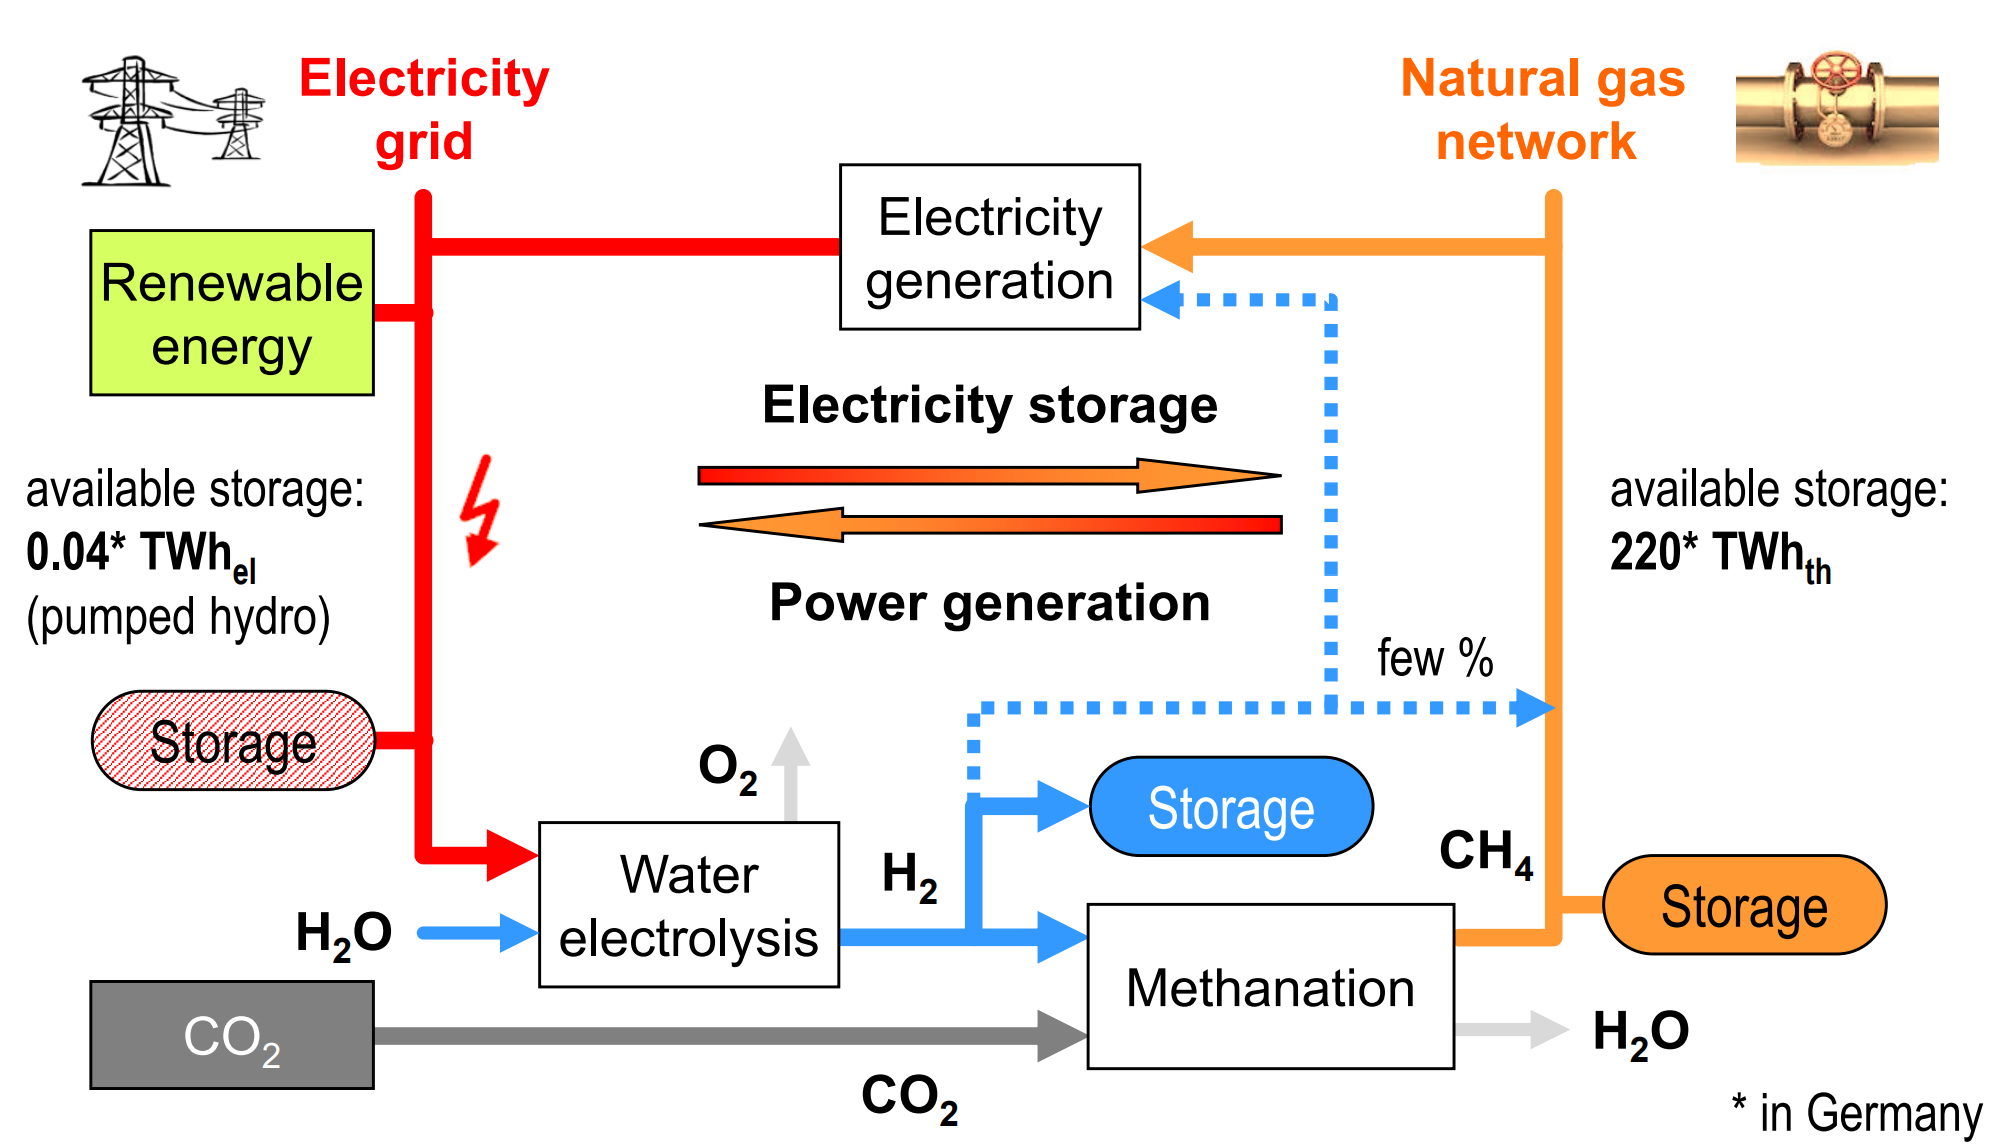
\includegraphics[width=0.75\linewidth]{src/p2g.png}
\end{figure}

\subsubsection{Methanation}
sabatier reaction: $$
\mathrm{CO}_2+4 \mathrm{H}_2 \rightarrow \mathrm{CH}_4+2 \mathrm{H}_2 \mathrm{O}(\mathrm{g}) \quad \Delta_{\mathrm{r}} \mathrm{H}^{\circ}=-165 \mathrm{~kJ} / \mathrm{mol}
$$ 
water-gas-shift: $\mathrm{CO} + \mathrm{H}_2\mathrm{O(g)} \leftrightarrow \mathrm{CO}_2 + \mathrm{H}_2 \quad \Delta_{\mathrm{r}} \mathrm{H}^{\circ}=-41 \mathrm{~kJ} / \mathrm{mol}$ \\
methanation: $\mathrm{CO} + 3\mathrm{H}_2 \rightarrow \mathrm{CH}_4 + \mathrm{H}_2\mathrm{O(g)} \quad \Delta_{\mathrm{r}} \mathrm{H}^{\circ}=-206 \mathrm{~kJ} / \mathrm{mol}$ \\
theoretical eff.:
$
\varepsilon_{\mathrm{th}}=\frac{L H V\left(\mathrm{CH}_4\right)}{4 \cdot L H V\left(\mathrm{H}_2\right)}=\frac{9.94 \mathrm{kWh} / \mathrm{Nm}^3}{4 \cdot 3.00 \mathrm{kWh} / \mathrm{Nm}^3}=82.8 \%
$ \\
there is a tradeoff of equilibrium vs. rate, at ($347^\circ\mathrm{C}, 6\mathrm{bar}$) the yield is largest (at +/- T: thermodynamic/kinetic limitation)

\subsubsection{comparison of product}
\tiny
\begin{tabular}{|p{.75cm}|p{3.8cm}|p{3.8cm}|}
\hline
\textbf{Gas} & \textbf{Advantage} & \textbf{Disadvantage} \\ \hline
$\mathrm{H_2}$ & - higher P2G conversion efficiency \newline
- no CO2 source required \newline
- carbon-free energy carrier \newline
- higher efficiency of re-electrification (e.g. in fuel cells) & 
- H2 less generic product than CH4 \newline
- Injection of excess H2 into natural gas grid limited \\ \hline
Methane & - more generic product than H2 \newline
- “green” methane can be produced (depending on the CO2 source)
- other uses of CH4 conceivable (industrial use) \newline
- injection into natural gas grid possible without limit & 
- lower conversion and round-trip efficiency \newline
- suitable CO2 source required (preferably “green” CO2) \newline
- cost of produced SNG not competitive with fossil natural gas (at the moment) \\ \hline
\end{tabular}

\small

\subsubsection{efficiency}
electricity $\Rightarrow$ $\mathrm{CH}_4$: heat in (electrolysis,  methanation) $\epsilon_1=60\%$ \\
$\mathrm{CH}_4$ $\Rightarrow$ electricity: combined cycle plant $\epsilon_2=60\%$ \\
bad total efficiency $\epsilon_{tot}=36\%\Rightarrow$ avoid P2G whenever possible

\subsubsection{energy density $\rho$}
can be measured by volume or mass \\
$\rho_{\text{gasoline}} \gg \rho_{\text{liquid $\mathrm{H}_2$}} > \rho_{\text{chem. hydrides}} > \rho_{\text{compr. gas $\mathrm{H}_2$}} \gg \rho_\text{batteries}$ \\
however, batteries make up for it with large total efficiency advantage, e.g. for vehicles: (69\% vs. 26\% vs. 13\% for $\eta_\text{bat},\eta_{\mathrm{H}_2},\eta_{\text{gasoline}}$)

\subsection{$\mathrm{CO_2}$ capture}
\subsubsection{$\mathrm{CO_2}$ sources}
\begin{tabular}{|p{1.2cm}|p{7.5cm}|}
\hline
\textbf{Source} & \textbf{Details} \\ \hline
Coal power plants & - separation from flue gas \newline
- fossil CO2 \newline
- cost: 30 – 80 \$ / tCO2 \newline
- energy input: 230 – 400 kWh / tCO2 \\ \hline
Air & - abundant \newline
- absorption with alkaline solutions \newline
- cost: 100 – 1'000 \$ / tCO2 \newline
- energy input: 1'200 – 2'500 kWh / tCO2 \\ \hline
Industrial processes & - cost and energy input dependent on process \newline
- large amounts theoretically available \newline
- ideally CO2 separation not necessary \\ \hline
\end{tabular}

\subsubsection{Gas Storage Capacity}
$>100\mathbf{GWh}$ in rock salt caverns and porous caverns. depending on location, power and storage capacity differ substantially.

\subsection{Power-to-X (P2X)}
general concept: linking power with other sectors \\
examples: Power-to-Heat, Power-to-generation, Power-to-Chemical industry, Power-to-fuel
\subsubsection{carbon intensive sectors}
chemicals, steel, cement heavily rely on fossil fuels and consume ~27 PWh/a of energy, corresponding to global annual electricity consumption
\subsubsection{Power-to-Liquid (P2L)}
steps: electricity $\xrightarrow{\mathrm{H}_2\mathrm{O}+\text{electrolyzer}} \mathrm{H}_2$ $\xrightarrow{\mathrm{CO}_2+\text{RWGS reactor}}$ $\mathrm{CO}/H_2$ supply $\xrightarrow{\text{Fischer-Tropsch reactor}}$ gas-to-liquid $\xrightarrow{\text{refining}}$ jet fuel 

% \section{Life Cycle Analysis (LCA)}
% Def.: LCA is a technique to assess environmental impacts associated with all the stages of a product's life cycle \textit{from-cradle-to-grave}, i.e., from raw material extraction through materials processing, manufacturing, distribution, use, repair and maintenance, and disposal or recycling.
% \vspace{-.5cm}
% \begin{figure}[H]
%     \centering
%     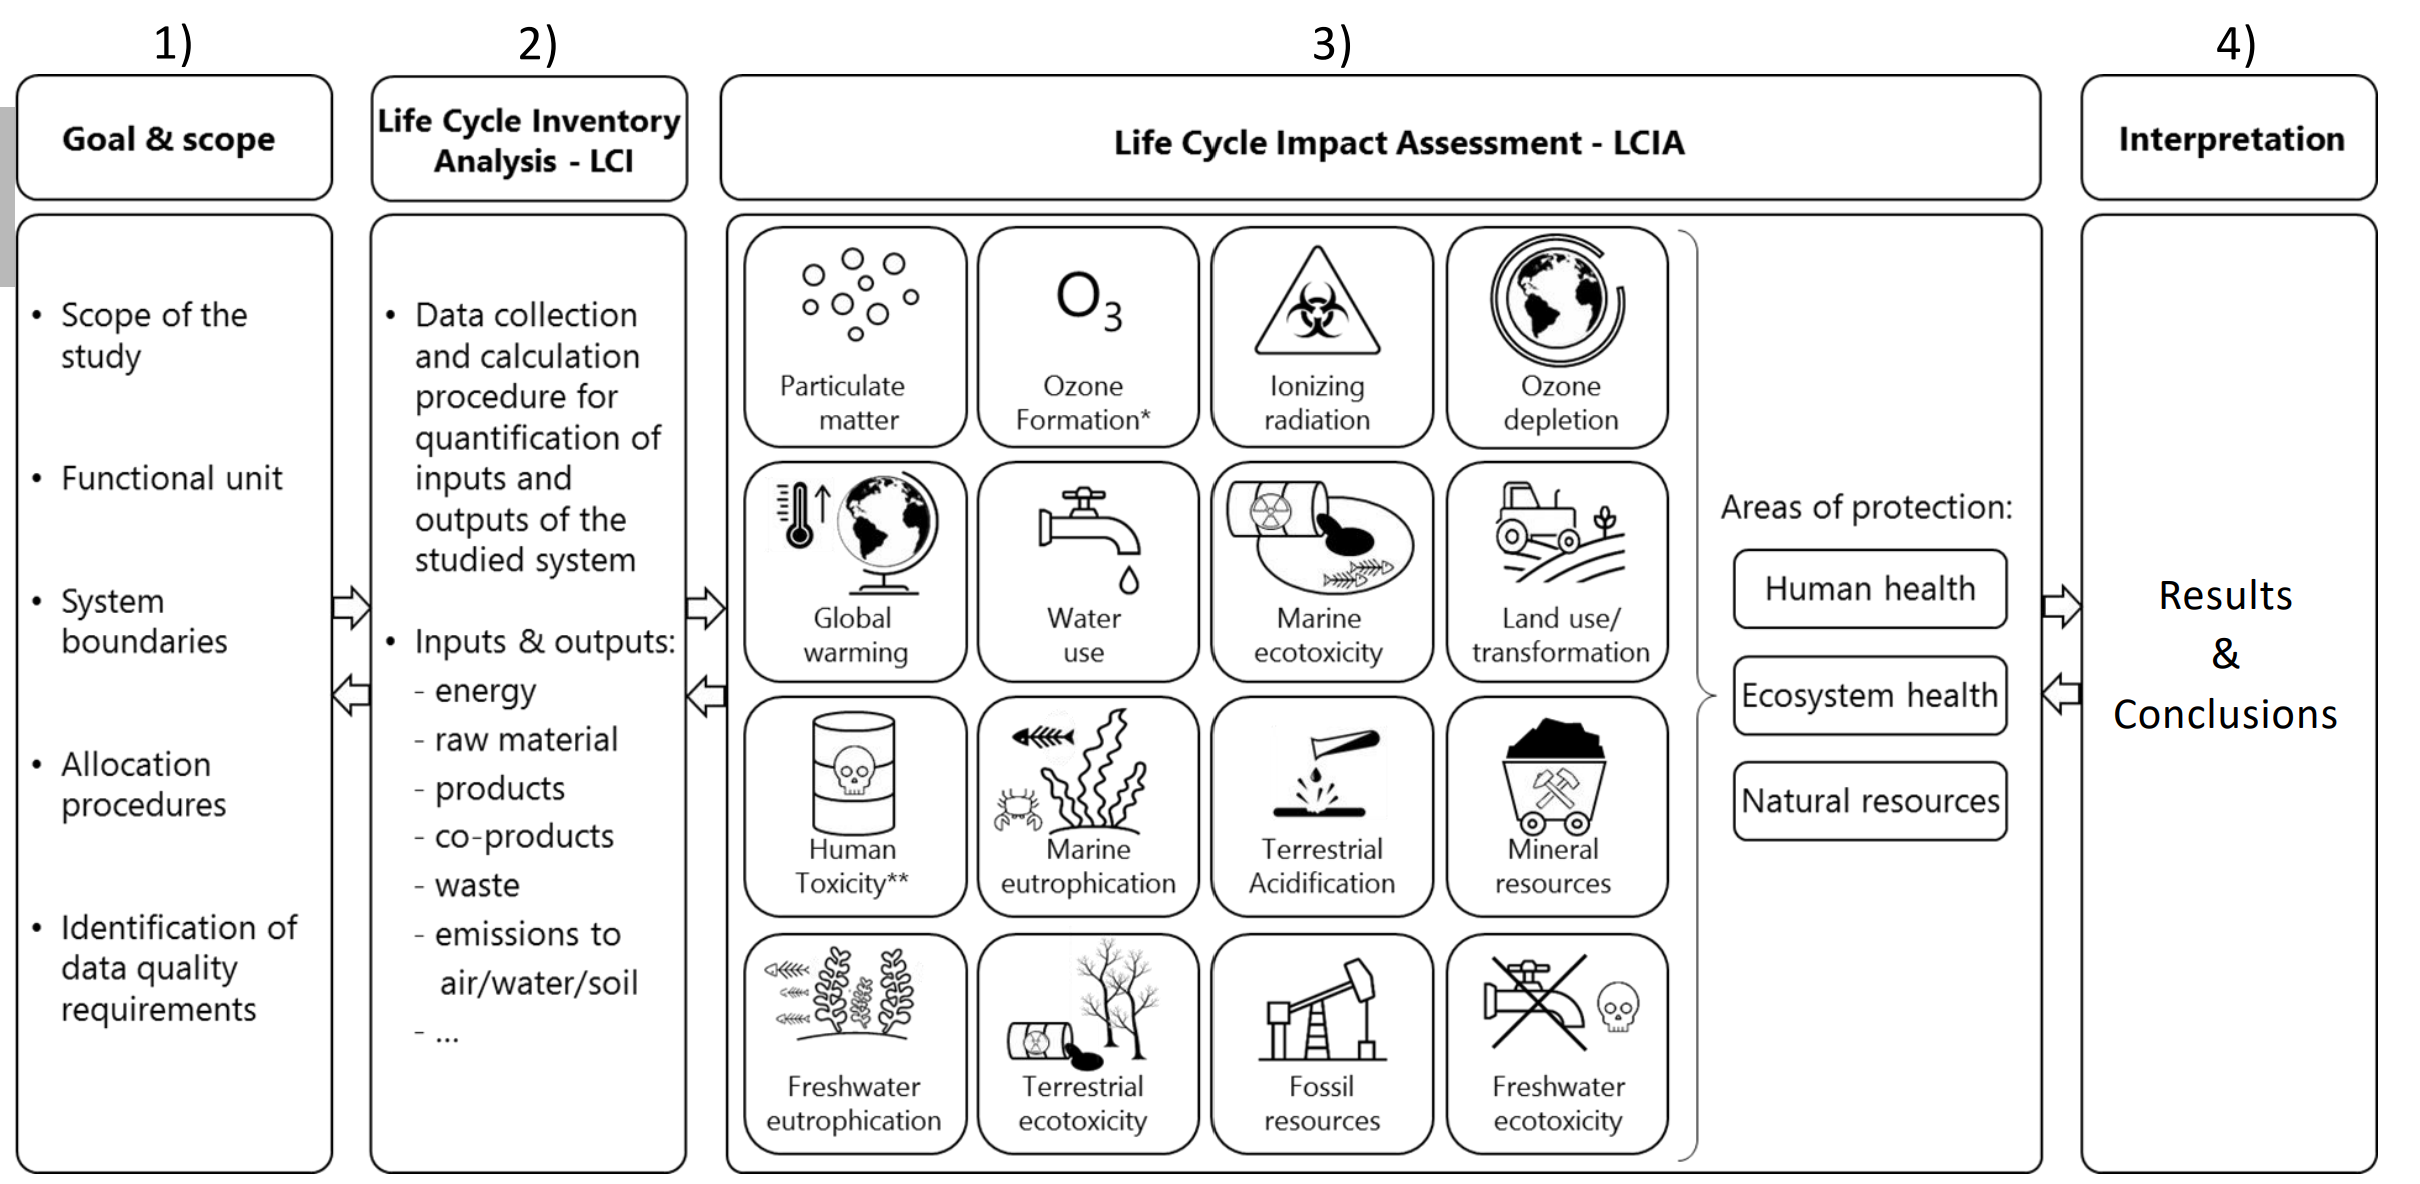
\includegraphics[width=1\linewidth]{src/LCA_overview.png}
% \end{figure}
% \vspace{-.5cm}

% \subsection{LCI}
% comprises LCI foreground data (often scope-specific date) and background data (often public database), evaluated via LCA software to yield LCA results.

% \subsection{LCIA}
% estimation of impacts and aggregation of LCI results into few indicators. \\
% goal: 1) estimation of overall human \& environmental impacts; 2) compact, illustrative \& understandable results \\
% methods: ReCiPe (midpoints, endpoints \& full aggregation), Environmental Footprint method, Ecological Scarcity

% \subsection{Energy related results}
% \subsubsection{batteries}
% around 1/2 reduction of GHG until 2050 to 45-55 $\mathrm{\frac{kg_{CO_2}}{kWh}}$

% \subsubsection{$\mathrm{H_2}$ based e-fuels}
% 2 (industrial heating) to 14 (residential heating) times more electricity and therefore environmental impact compared to direct electrification

% \subsubsection{$\mathrm{H_2}$ production}
% with today's electricity mix or methods, $\mathrm{H_2}$ production is climate harming. if only RE is used or high-CCS ($>90\%$ capture rate) + low leakage of $\mathrm{CH_4}$

% \subsection{limitations of LCA}
% \begin{itemize}
%     \item Economic \& social factors are \textbf{not} included
%     \item LCA addresses only environmental impacts from “normal operation” (Accidents are \textbf{not} included)
%     \item Limited coverage of global production chains
% \end{itemize}

% \section{Energy Modeling}
% Def.: A scenario is a \textit{plausible description} of how the future may develop, based on a coherent and internally consistent set of \textit{assumptions} (“scenario logic”) about key relationships and driving forces (e.g., rate of technology changes, prices). \\
% neither \textbf{predictions nor forecasts}

% \subsection{types of models}
% \begin{figure}[H]
%     \centering
%     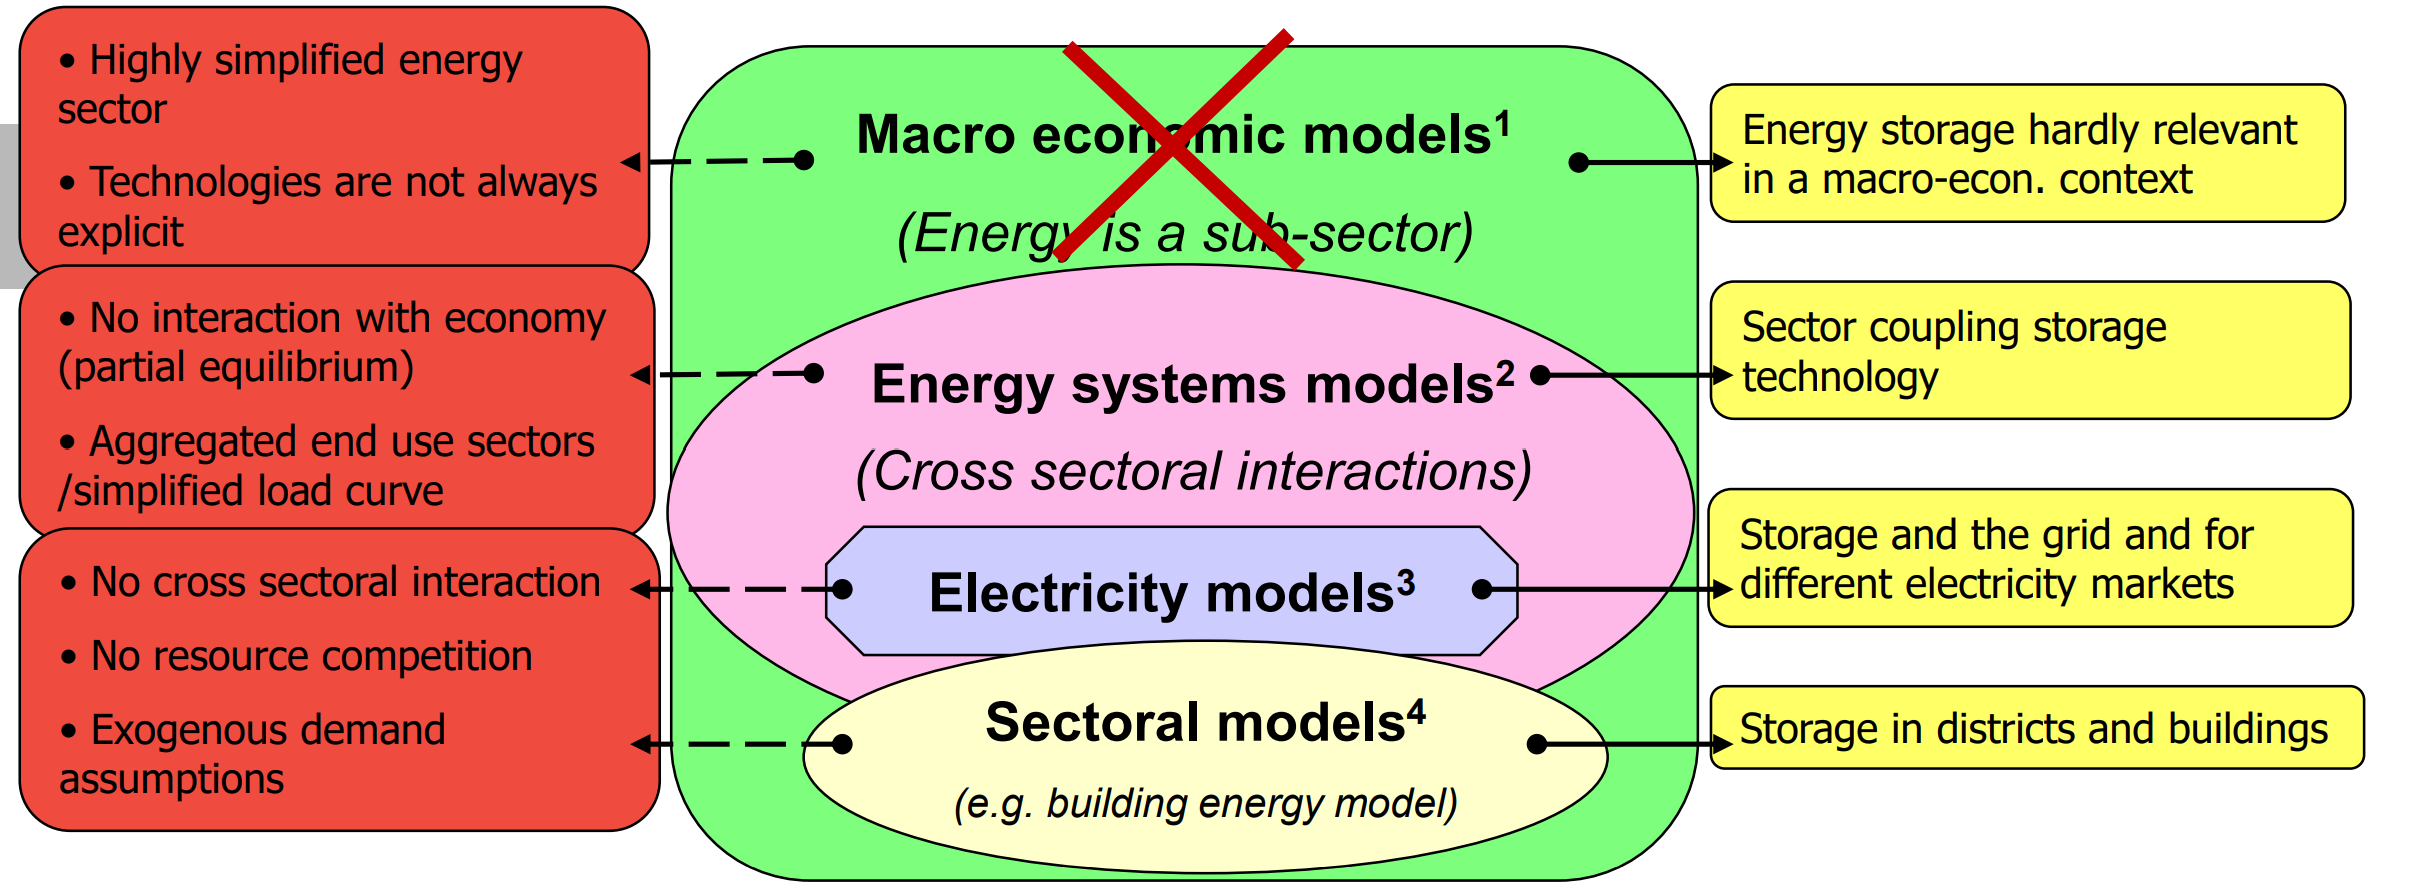
\includegraphics[width=1\linewidth]{src/energy_models.png}
% \end{figure}
% there are trade-offs which model is most useful, depending on scope and objective.

% \subsection{temporal clustering}
% 1.\textit{averaging}: avg. values of time frame \\
% 2.\textit{representative days}: pick small number of representative time frames \\
% the 2. approach is more accurate in energy context.

% \subsection{typical model}
% \begin{align*}
%     \min \quad& I_c + C_{O\&M} + C_{fuel} + ... \\
%     \mathrm{s.t.} \quad& \text{availability of tech., potential} \\
%     & \text{balance equ. potentials of energy carriers} \\
%     & \text{reserve capacity, } \text{policy constraints} \\
%     & \dots \\
%     \text{variables}\quad & \text{investment, capacity, output per technology} \\
%     & \text{imports/exports of energy carriers} \\
%     & \dots
% \end{align*}

% \subsection{Economic rationale}
% Partial equilibrium model (simultaneously configuration of production and consumption and the corresponding prices) \\
% Maximization of total surplus: Price equals marginal value \\

% \subsection{results for RE}
% 4-flexibility options to integrate RE effectively:
% \begin{itemize}
%     \item electricity storage
%     \item heat storage and load shifting
%     \item smart transport electrification
%     \item sector coupling via P2G
% \end{itemize}



\section{Energy System Challenges}
\section{global overview}
fossil fuel account for roughly 82\% of total energy demand. RE at $7.5\%$ and hydro at $6.6\%$ \\
R/P ratio: represent the length of time that those remaining reserves would last,  if production were to continue at the previous year’s rate: \\
\begin{tabular}{|p{1cm}|p{2cm}|p{2cm}|p{2cm}|}
         & Oil & Gas & coal \\
    R\&P & 50y & 48.8 & 139 \\
    $\mathrm{\frac{MWh}{barrel}}$ & 1.7 & & \\
\end{tabular}
\begin{tabular}{|p{1cm}|p{2cm}|p{2cm}|p{2cm}|}
         & Gasoline & Ethanol & ... \\
    $\mathrm{\frac{kg_{CO2}}{l_x}}$ & 2.353 & 1.524 
\end{tabular}
    

\subsection{climate change}
climate change main reason to ditch fossil fuels \\
neagtive impacts:
\begin{itemize}
    \item Decrease availability of water and increase drought at mid-latitudes
    \item Disruption of ecosystems and extinction of species
    \item Changes in the carbon cycle
    \item Acidification of the ocean
    \item Decrease of food-crop productivity
    \item Loss of wetlands 
\end{itemize}

\subsection{decarbonization}
Def.: decoupling of $\mathrm{CO_2}$ and energy production. \\
through: efficiency, low-carbon energy sources, CCUS (lol) \\

\subsection{renewables (RE)}
come from natural sources or processes \textit{constantly naturally replenished} (hydro, solar, wind, biomass, tidal, ...) \\
are intermittent \\
\textbf{ bio-ethanol} is a combustion process. However, the plants used for the production of bio-ethanol can be grown every year using sun as energy and they can regrow in a relatively short time, thus its renewable.

\subsection{examples}
What is area needed to replace fuel with bio-ethano?
$A=\mathrm{\frac{1 l_{eth}}{0.67 l_{gas}}\cdot 10^{10} kg_{gas}\cdot\frac{10^3 l_{gas}}{850 kg_{gas}}\cdot\frac{m^2}{37.5\cdot10^{-2}l_{eth}}}$



\section{appendix}
\subsection{equations}
\noindent
\begin{tabular}{|p{2cm}|p{4.5cm}|p{1.5cm}|}
\textbf{name} & \textbf{equ.} & \textbf{(unit)} \\
\hline
$T_0$ & 298.15 / 25 & K / $^\circ C$ \\
$p_0$ &  1.01325 / 1 & bar / atm \\
activity &  $a=1$ & \\
concentration & $c_0=1$ & $\frac{\text{mol}}{\text{L}}$ \\
activity for ionic species & $a=\frac{\gamma\cdot c}{c_0}$ & \\
ideal gas & $pV=nRT$ & \\

\end{tabular}

\subsection{Standard Electrode Potentials}
for $T_0, p_0, a$: \\
\begin{tabular}{|p{4cm}|p{4cm}|}
\hline
\textbf{Half-cell reaction} & \textbf{E\(^\circ\) (V vs. SHE)} \\ \hline
F\(_2\) + 2 e\(^-\) → 2 F\(^-\) & +2.87 \\ \hline
Ce\(^{4+}\) + e\(^-\) → Ce\(^{3+}\) & +1.61 \\ \hline
MnO\(_4^-\) + 8 H\(^+\) + 5 e\(^-\) → Mn\(^{2+}\) + 4 H\(_2\)O & +1.51 \\ \hline
Cl\(_2\) + 2 e\(^-\) → 2 Cl\(^-\) & +1.36 \\ \hline
Cr\(_2\)O\(_7^{2-}\) + 14 H\(^+\) + 6 e\(^-\) → 2 Cr\(^{3+}\) + 7 H\(_2\)O & +1.33 \\ \hline
O\(_2\) + 4 H\(^+\) + 4 e\(^-\) → 2 H\(_2\)O & +1.23 \\ \hline
MnO\(_2\) + 4 H\(^+\) + 2 e\(^-\) → Mn\(^{2+}\) + 2 H\(_2\)O & +1.23 \\ \hline
Br\(_2\) + 2 e\(^-\) → 2 Br\(^-\) & +1.06 \\ \hline
NO\(_3^-\) + 4 H\(^+\) + 3 e\(^-\) → NO + H\(_2\)O & +0.96 \\ \hline
Ag\(^+\) + e\(^-\) → Ag & +0.80 \\ \hline
Fe\(^{3+}\) + e\(^-\) → Fe\(^{2+}\) & +0.77 \\ \hline
Q + 2 H\(^+\) + 2 e\(^-\) → H\(_2\)Q (*) & +0.699 \\ \hline
O\(_2\) + 2 H\(^+\) + 2 e\(^-\) → H\(_2\)O\(_2\) & +0.68 \\ \hline
MnO\(_4^-\) + 2 H\(_2\)O + 3 e\(^-\) → MnO\(_2\) + 4 OH\(^-\) & +0.59 \\ \hline
I\(_2\) + 2 e\(^-\) → 2 I\(^-\) & +0.54 \\ \hline
O\(_2\) + 2 H\(_2\)O + 4 e\(^-\) → 4 OH\(^-\) & +0.40 \\ \hline
[Fe(CN)\(_6\)]\(^{3-}\) + e\(^-\) → [Fe(CN)\(_6\)]\(^{4-}\) & +0.370 \\ \hline
Cu\(^{2+}\) + 2 e\(^-\) → Cu & +0.34 \\ \hline
AgCl(s) + e\(^-\) → Ag + Cl\(^-\) & +0.222 \\ \hline
\textbf{2 H\(^+\) + 2 e\(^-\) → H\(_2\)} & \textbf{0.00} \\ \hline
Ni\(^{2+}\) + 2 e\(^-\) → Ni & –0.28 \\ \hline
Cd\(^{2+}\) + 2 e\(^-\) → Cd & –0.40 \\ \hline
Fe\(^{2+}\) + 2 e\(^-\) → Fe & –0.44 \\ \hline
Zn\(^{2+}\) + 2 e\(^-\) → Zn & –0.76 \\ \hline
2 H\(_2\)O + 2 e\(^-\) → H\(_2\) + 2 OH\(^-\) & –0.83 \\ \hline
Al\(^{3+}\) + 3 e\(^-\) → Al & –1.66 \\ \hline
Na\(^+\) + e\(^-\) → Na & –2.71 \\ \hline
Li\(^+\) + e\(^-\) → Li & –3.05 \\ \hline
\end{tabular}

\subsection{matric prefixes}
\begin{tabular}{|c|c|c|c|}
\hline
\textbf{Prefix} & \textbf{Symbol} & \textbf{Factor} & \textbf{Power} \\ \hline
peta  & P   & 1000000000000  & $10^{15}$  \\ \hline
tera  & T   & 1000000000000  & $10^{12}$  \\ \hline
giga  & G   & 1000000000  & $10^{9}$  \\ \hline
mega  & M   & 1000000  & $10^{6}$  \\ \hline
kilo  & k   & 1000  & $10^{3}$  \\ \hline
hecto & h   & 100  & $10^{2}$  \\ \hline
deca  & da  & 10  & $10^{1}$  \\ \hline
(none) & (none) & 1  & $10^{0}$  \\ \hline
deci  & d   & 0.1  & $10^{-1}$ \\ \hline
centi & c   & 0.01  & $10^{-2}$ \\ \hline
milli & m   & 0.001  & $10^{-3}$ \\ \hline
micro & $\mu$ & 0.000001 & $10^{-6}$ \\ \hline
nano  & n   & 0.000000001  & $10^{-9}$ \\ \hline
pico  & p   & 0.000000000001  & $10^{-12}$ \\ \hline
\end{tabular}

\subsection{oxidation \#}
\begin{table}[H]
\centering
\begin{tabular}{|l|l|l|}
\hline
\textbf{Element}           & \textbf{Oxidation \#} & \textbf{Exceptions}                        \\ \hline
Group 1 metals             & Always +1                      &                                            \\ \hline
Group 2 metals             & Always +2                      &                                            \\ \hline
$\mathrm{O}$                     & Usually -2                     & Peroxides and F$_2$O            \\ \hline
$\mathrm{H}$                   & Usually +1                     & Metal hydrides (-1)             \\ \hline
Fluorine                   & Always -1                      &                                            \\ \hline
Chlorine                   & Usually -1                     & Compounds with O or F           \\ \hline
\end{tabular}
\label{table:oxidation_states}
\end{table}
\section{Disclaimer}

This summary was created by Carl von Holly-Ponientzietz. There is no guarantee of correctness. This summary can be reused under the condition that it is shared with students on AMIV.

\end{multicols*}


%

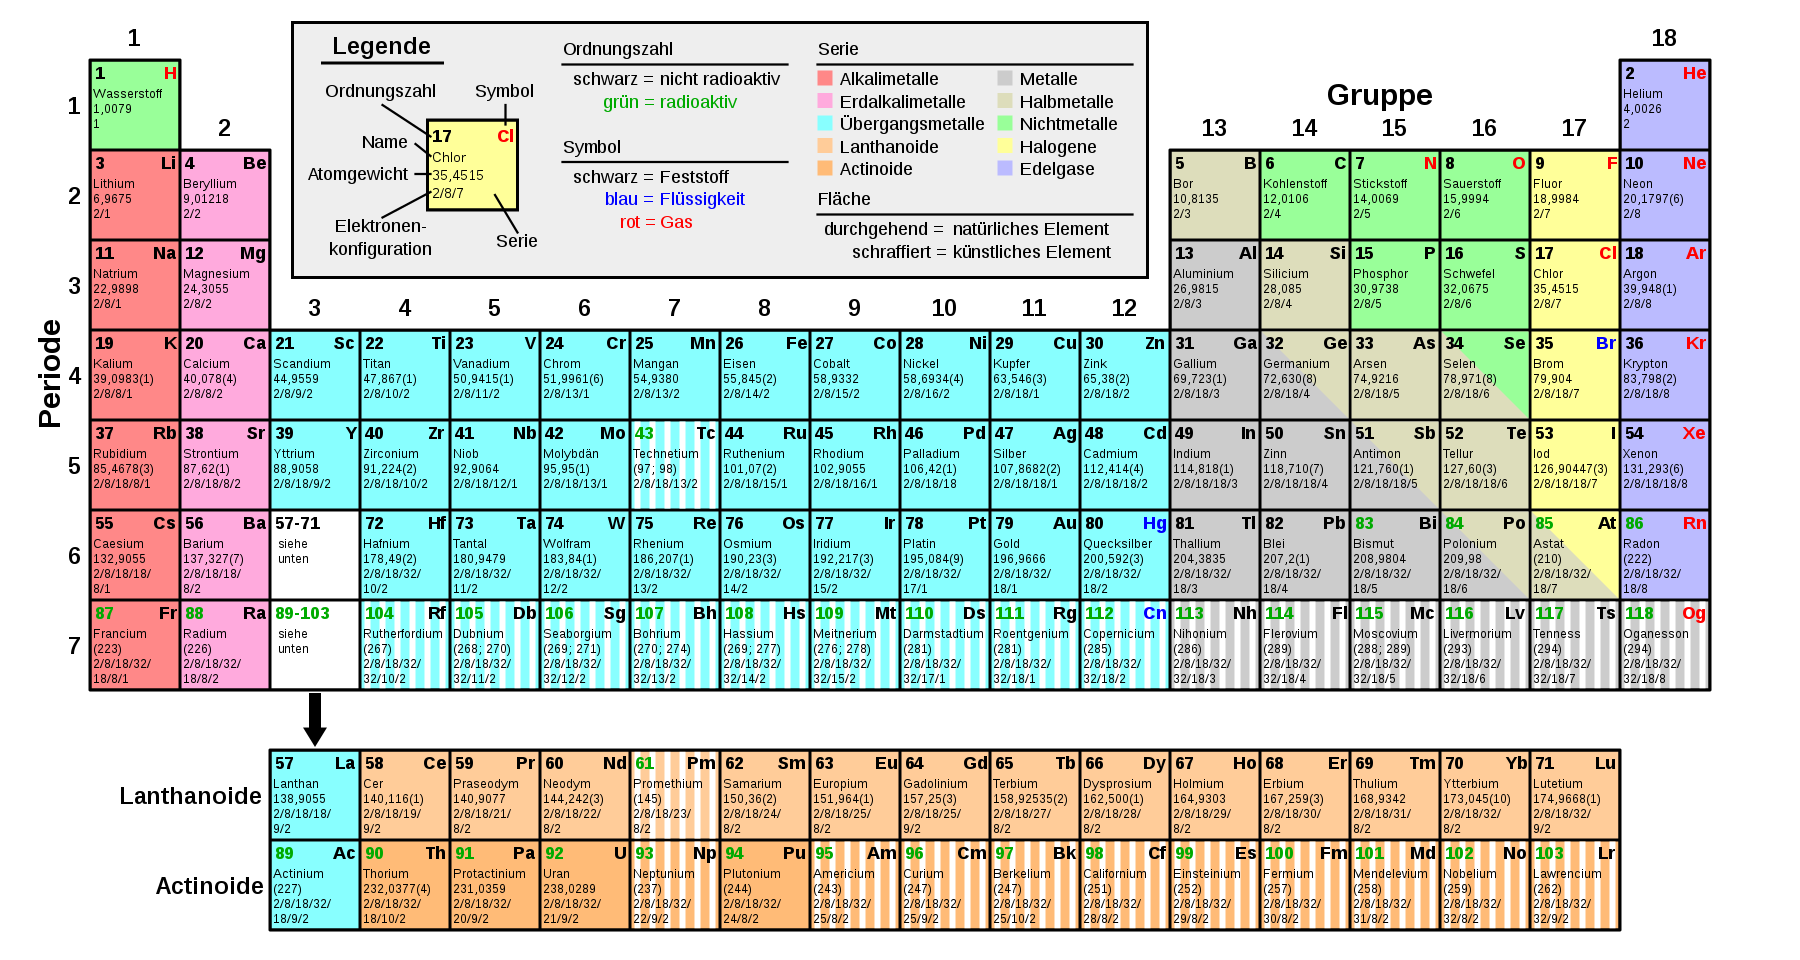
\includegraphics[width = 1.03\textwidth]{src/periodictable.png}

\end{document}